% !TeX spellcheck = en_US
\documentclass[hidelinks,titlepage,a4paper]{article}

\usepackage[utf8]{inputenc}
\usepackage[T1]{fontenc}
\usepackage{lmodern}
\usepackage{newpxtext,newpxmath}
\linespread{1.05} % Line spacing - Palatino needs more space between lines
\usepackage{microtype}
\usepackage[group-separator={,}]{siunitx}
\usepackage[tikz]{bclogo}
\usepackage{pgfplots}
\usepackage{appendix}
\usepackage{verbatim}
\usepackage[hyphens]{url}
\usepackage{hyperref} % For hyperlinks in the PDF
\usepackage{fontawesome5}
\usepackage[os=win]{menukeys}

\usepackage[hmarginratio=1:1,top=32mm,columnsep=20pt]{geometry} % Document margins
\geometry{a4paper,textwidth=6.5in,hmarginratio=1:1,
  textheight=9in,vmarginratio=1:1,heightrounded}

\usepackage{titlesec}
\setcounter{secnumdepth}{4}
\setcounter{tocdepth}{4}

\titleformat{\paragraph}
{\normalfont\normalsize\bfseries}{\theparagraph}{1em}{}
\titlespacing*{\paragraph}
{0pt}{3.25ex plus 1ex minus .2ex}{1.5ex plus .2ex}

\usepackage{fancyhdr} % Headers and footers
\pagestyle{fancy} % All pages have headers and footers
\fancyhead{} % Blank out the default header
\fancyfoot{} % Blank out the default footer
\fancyhead[L]{Tracy Profiler}
\fancyhead[R]{The user manual}
\fancyfoot[RO]{\thepage} % Custom footer text

\usepackage{listings}
\usepackage{xcolor}
\usepackage{float}
\lstset{language=C++}
\lstset{
         basicstyle=\footnotesize\ttfamily,
         tabsize=4,
         extendedchars=true,
         breaklines=true,
         stringstyle=\ttfamily,
         showspaces=false,
         xleftmargin=17pt,
         framexleftmargin=17pt,
         framexrightmargin=5pt,
         framexbottommargin=4pt,
         showstringspaces=false,
         escapeinside={@}{@},
         aboveskip=0pt,
         belowskip=\baselineskip
}

\usepackage[hang, small,labelfont=bf,up,textfont=it,up]{caption} % Custom captions under/above floats in tables or figures

\usepackage{tikz}
\usetikzlibrary{arrows.meta,positioning,shapes,patterns}

\newcommand{\LMB}{
\includegraphics[height=.8\baselineskip]{icons/lmb}}
\newcommand{\RMB}{
\includegraphics[height=.8\baselineskip]{icons/rmb}}
\newcommand{\MMB}{
\includegraphics[height=.8\baselineskip]{icons/mmb}}
\newcommand{\Scroll}{
\includegraphics[height=.8\baselineskip]{icons/scroll}}

\newcommand*\circled[1]{\tikz[baseline=(char.base)]{
    \node[shape=circle,draw,inner sep=1.5pt] (char) {#1};}}

\begin{document}

\begin{titlepage}
\centering
{\fontsize{120}{140}\selectfont Tracy Profiler}

\vspace{50pt} {\Huge\fontfamily{lmtt}\selectfont The user manual}
\vfill
\large\textbf{Bartosz Taudul} \href{mailto:wolf.pld@gmail.com}{<wolf.pld@gmail.com>}

\vspace{10pt}
\today
\vfill
\url{https://bitbucket.org/wolfpld/tracy}
\end{titlepage}

\tableofcontents

\newpage

\section{A quick look at Tracy}

Tracy is a real-time, nanosecond resolution \emph{frame profiler} that can be used for remote or embedded telemetry of applications. It can profile CPU (C, C++11, Lua), GPU (OpenGL, Vulkan) and memory. It also can monitor locks held by threads and show where contention does happen.

In contrast with \emph{statistical profilers} (such as VTune, perf or Very Sleepy), Tracy does require manual markup of the source code. In return, it allows frame-by-frame inspection of the program execution. You will be able to see exactly which functions are called, how much time is spent in them, and how do they interact with each other in a multi-threaded environment. This feat is by-design impossible to achieve in statistical profilers, which work by periodically sampling the \emph{program counter} register to see which part of the code is executing.

Even though Tracy is a \emph{frame} profiler, with the emphasis on analysis of \emph{frame time} in real-time applications, it does work with utilities that do not employ the concept of a frame. There's nothing that would prohibit profiling of, for example, a compression tool, or an event-driven UI application.

The close analogues of Tracy are: RAD Telemetry, Brofiler, microprofile.

Now let's take a close look at the marketing blurb.

\subsection{Real-time}

This claim can be described in the following ways:

\begin{enumerate}
\item The profiled application is not slowed down by profiling\footnote{See section~\ref{perfimpact} for a benchmark.}. The act of recording a profiling event has virtually zero cost -- it only takes \textasciitilde 8~\si{\nano\second}. Even on low-power mobile devices there's no perceptible impact on execution speed.
\item The profiler itself works in real-time, without the need to process collected data in a complex way. Actually, it is quite inefficient in the way it works, as the data it presents is calculated anew each frame. And yet it can run at 60 frames per second.
\item The profiler has full functionality when the profiled application is running and the data is captured. You may interact with your application and then immediately switch to the profiler, when a performance drop occurs.
\end{enumerate}

\subsection{Nanosecond resolution}

It is hard to imagine how long a nanosecond is. One good analogy is to compare it with a measure of length. Let's say that one second is one meter (the average doorknob is on the height of one meter).

One millisecond ($\frac{1}{1000}$ of a second) would be then the length of a millimeter. The average size of a red ant or the width of a pencil is 5 or 6~\si{\milli\metre}. A modern game running at 60 frames per second has only 16~\si{\milli\second} to update the game world and render the entire scene.

One microsecond ($\frac{1}{1000}$ of a millisecond) in our comparison equals to one micron. The diameter of a typical bacterium ranges from 1 to 10 microns. The diameter of a red blood cell, or width of strand of spider web silk is about 7~\si{\micro\metre}.

And finally, one nanosecond ($\frac{1}{1000}$ of a microsecond) would be one nanometer. The modern microprocessor transistor gate, the width of DNA helix, or the thickness of a cell membrane are in the range of 5~\si{\nano\metre}. In one~\si{\nano\second} the light can travel only 30~\si{\centi\meter}.

Tracy can achieve single-digit nanosecond measurement resolution, due to usage of hardware timing mechanisms on the x86 and ARM architectures\footnote{In both 32 and 64~bit variants. On x86 Tracy requires a modern version of the \texttt{rdtscp} instruction (Sandy Bridge and later). On ARM-based systems Tracy will try to use the timer register (\textasciitilde 40 \si{\nano\second} resolution). If it fails (due to kernel configuration), Tracy falls back to system provided timer, which can range in resolution from 250 \si{\nano\second} to 1 \si{\micro\second}.}. Other profilers may rely on the timers provided by operating system, which do have significantly reduced resolution (about 300~\si{\nano\second} -- 1~\si{\micro\second}). This is enough to hide the subtle impact of cache access optimization, etc.

\subsubsection{Timer accuracy}

You may wonder why it is important to have a high resolution timer\footnote{Interestingly, the \texttt{std::chrono::high\_resolution\_clock} is not really a high resolution clock.}. After all, you only want to profile functions that have long execution times, and not some short-lived procedures, that have no impact on the application's run time.

It is wrong to think so. Optimizing a function to execute in 430~\si{\nano\second}, instead of 535~\si{\nano\second} (note that there is only a 100~\si{\nano\second} difference) results in 14 \si{\milli\second} savings if the function is executed 18000 times\footnote{This is a real optimization case. The values are median function run times and do not reflect the real execution time, which explains the discrepancy in the total reported time.}. It may not seem like a big number, but this is how much time there is to render a complete frame in a 60~FPS game. Imagine that this is your particle processing loop.

You also need to understand how timer precision is reflected in measurement errors. Take a look at figure~\ref{timer}. There you can see three discrete timer tick events, which increase the value reported by the timer by 300~\si{\nano\second}. You can also see four readings of time ranges, marked $A_1$, $A_2$; $B_1$, $B_2$; $C_1$, $C_2$ and $D_1$, $D_2$.

\begin{figure}[h]
\centering\begin{tikzpicture}
\draw [-{Stealth}] (-1.5, 0) -- (11.5, 0) node[anchor=south east] {Time};
\draw (0, -0.25) -- (0, 0.25) node[anchor=south] {\faClock};
\draw (5, -0.25) -- (5, 0.25) node[anchor=south] {\faClock};
\draw (10, -0.25) -- (10, 0.25) node[anchor=south] {\faClock};
\draw (0, 0.9) -- (0, 1) -- (5, 1) -- (5, 0.9);
\draw (2.5, 1) node[anchor=south] {300~\si{\nano\second}};

\draw (4.9, 0.1) -- (4.9, -0.1);
\draw [{Stealth}-] (4.9, -0.2) -- (4.8, -0.7) node[anchor=north] {$A_1$};
\draw (5.1, 0.1) -- (5.1, -0.1);
\draw [{Stealth}-] (5.1, -0.2) -- (5.2, -0.7) node[anchor=north] {$A_2$};

\draw (0.1, 0.1) -- (0.1, -0.1);
\draw [{Stealth}-] (0.1, -0.2) -- (0.2, -0.7) node[anchor=north] {$B_1$};
\draw (9.9, 0.1) -- (9.9, -0.1);
\draw [{Stealth}-] (9.9, -0.2) -- (9.8, -0.7) node[anchor=north] {$B_2$};

\draw (-0.1, 0.1) -- (-0.1, -0.1);
\draw [{Stealth}-] (-0.1, -0.2) -- (-0.2, -0.7) node[anchor=north] {$C_1$};
\draw (10.1, 0.1) -- (10.1, -0.1);
\draw [{Stealth}-] (10.1, -0.2) -- (10.2, -0.7) node[anchor=north] {$C_2$};

\draw (2.4, 0.1) -- (2.4, -0.1);
\draw [{Stealth}-] (2.4, -0.2) -- (2.3, -0.7) node[anchor=north] {$D_1$};
\draw (2.6, 0.1) -- (2.6, -0.1);
\draw [{Stealth}-] (2.6, -0.2) -- (2.7, -0.7) node[anchor=north] {$D_2$};
\end{tikzpicture}
\caption{Low precision (300~ns) timer. Discrete timer ticks are indicated by the \faClock{} icon.}
\label{timer}
\end{figure}

Now let's take a look at the timer readings.

\begin{itemize}
\item The $A$ and $D$ ranges both take a very short amount of time (10~\si{\nano\second}), but the $A$ range is reported as 300~\si{\nano\second}, and the $D$ range is reported as 0~\si{\nano\second}.
\item The $B$ range takes a considerable amount of time (590~\si{\nano\second}), but according to the timer readings, it took the same time (300~\si{\nano\second}) as the short lived $A$ range.
\item The $C$ range (610~\si{\nano\second}) is only 20~\si{\nano\second} longer than the $B$ range, but it is reported as 900~\si{\nano\second}, a 600~\si{\nano\second} difference!
\end{itemize}

Here you can see why it is important to use a high precision timer. While there is no escape from the measurement errors, their impact can be reduced by increasing the timer accuracy.

\subsection{Frame profiler}

Tracy is aimed at understanding the inner workings of a tight loop of a game (or an interactive application). That's why it slices the execution time of a program using the \emph{frame}\footnote{A frame is used to describe a single image displayed on the screen by the game (or any other program), preferably 60 times per second to achieve smooth animation. You can also think about physics update frames, audio processing frames, etc.} as a basic work-unit\footnote{Frame usage is not required. See section~\ref{markingframes} for more information.}. The most interesting frames are the ones that took longer than the allocated time, producing visible hitches in the on-screen animation. Tracy allows inspection of such misbehavior.

\subsection{Remote or embedded telemetry}

Tracy uses the client-server model to enable a wide range of use-cases (see figure~\ref{clientserver}). For example, a game on a mobile phone may be profiled over the wireless connection, with the profiler running on a desktop computer. Or you can run the client and server on the same machine, using a localhost connection. It is also possible to embed the visualization front-end in the profiled application, making the profiling self-contained\footnote{See section~\ref{embeddingserver} for guidelines.}.

\begin{figure}[h]
\centering\begin{tikzpicture}
[inner sep=1.5mm, bend angle=30,
 thread/.style={rectangle, draw},
 module/.style={rectangle, draw, rounded corners=8pt},
 collect/.style={{Stealth}-, shorten <=4pt, shorten >=4pt},
 network/.style={cloud, draw, cloud ignores aspect, cloud puffs=11.6}]

\node[thread] (t1) {\faRandom{} Thread 1};
\node[thread] (t2) [below=of t1] {\faRandom{} Thread 2};
\node[thread] (t3) [below=of t2] {\faRandom{} Thread 3};

\node[module] (client) [right=of t2] {Tracy client}
	edge [collect, bend right] (t1)
	edge [collect] (t2)
	edge [collect, bend left] (t3);

\node[network] (network) [right=of client] {Network}
	edge [collect] (client);

\node[module] (server) [right=of network] {Tracy server}
	edge [collect] (network);

\begin{scope}[node distance=12pt, bend angle=25]
\node[thread] (display) [above right=of server] {\faTv{} Display}
	edge [collect, bend right] (server);
\node[thread] (storage) [below right=of server] {\faDatabase{} Storage}
	edge [collect, bend left] (server);
\end{scope}
\end{tikzpicture}
\caption{Client-server model.}
\label{clientserver}
\end{figure}

In Tracy terminology, the profiled application is a \emph{client} and the profiler itself is a \emph{server}. It was named this way because the client is a thin layer that just collects events and sends them for processing and long-term storage on the server. The fact that the server needs to connect to the client to begin the profiling session may be a bit confusing at first.

\subsection{Performance impact}
\label{perfimpact}

To check how much slowdown is introduced by using Tracy, let's profile an example application. For this purpose we will use etcpak\footnote{\url{https://bitbucket.org/wolfpld/etcpak}}. Let's use an $8192 \times 8192$ pixels test image as input data and instrument everything down to the $4 \times 4$ pixel block compression function (that's 4 million blocks to compress).

The resulting timing information can be seen in table~\ref{PerformanceImpact}. As can be seen, the cost of a single-zone capture (consisting of the zone begin and zone end events) is \textasciitilde 15 \si{\nano\second}.

\begin{table}[h]
\centering
\begin{tabular}[h]{c|c|c|c|c}
\textbf{Output} & \textbf{Zones} & \textbf{Clean run} & \textbf{Profiling run} & \textbf{Difference} \\ \hline
ETC1 & \num{4194568} & 0.94 \si{\second} & 1.003 \si{\second} & +0.063 \si{\second} \\
ETC2 + mip-maps & \num{5592822} & 1.034 \si{\second} & 1.119 \si{\second} & +0.085 \si{\second}
\end{tabular}
\caption{Zone capture time cost.}
\label{PerformanceImpact}
\end{table}

It should be noted that Tracy has a constant initialization cost, needed to perform timer calibration. This cost was subtracted from the profiling run times, as it is irrelevant to the single-zone capture time.

\section{First steps}

The following compilers are supported:

\begin{itemize}
\item MSVC
\item gcc
\item clang
\end{itemize}

The following platforms are confirmed to be working (this is not a complete list):

\begin{itemize}
\item Windows (x86, x64)
\item Linux (x86, x64, ARM, ARM64)
\item Android (ARM, x86)
\item FreeBSD (x64)
\item Cygwin (x64)
\item WSL (x64)
\item OSX (x64)\footnote{Be aware that support for Thread Local Storage is required. It is only available since Xcode 8 and not before iOS 9.}
\end{itemize}

\subsection{Initial client setup}

The recommended way to integrate Tracy into an application is to create a git submodule in the repository (assuming that git is used for version control). This way it is very easy to update Tracy to newly released versions.

If that's not an option, copy all files from the Tracy checkout directory to your project. Next, add the \texttt{tracy/TracyClient.cpp} source file to the IDE project and/or makefile. That's all. Tracy is now integrated into the application.

In the default configuration Tracy is disabled. This way you don't have to worry that the production builds will perform collection of profiling data. You will probably want to create a separate build configuration, with the \texttt{TRACY\_ENABLE} define, which enables profiling.

Finally, on Unix make sure that the application is linked with libraries \texttt{libpthread} and \texttt{libdl}.

\subsubsection{Short-lived applications}

In case you want to profile a short-lived program (for example, a compression utility that finishes its work in one second), add the \texttt{TRACY\_NO\_EXIT} define to the build configuration. With this option enabled, Tracy will not exit until an incoming connection is made, even if the application has already finished executing. This mode of operation can also be turned on by setting the \texttt{TRACY\_NO\_EXIT} environment variable to $1$.

\subsubsection{On-demand profiling}
\label{ondemand}

By default Tracy will begin profiling even before the program enters the \texttt{main} function. If you don't want to perform a full capture of application life-time, you may define the \texttt{TRACY\_ON\_DEMAND} macro, which will enable profiling only when there's an established connection with the server.

It should be noted, that if on-demand profiling is \emph{disabled} (which is the default), then the recorded events will be stored in the system memory until a server connection is made and the data can be uploaded\footnote{This memory is never released, but it is reused for collection of further events.}. Depending on the amount of the things profiled, the requirements for event storage can easily grow up to a couple of gigabytes. Since this data is cleared after the initial connection is made, you won't be able to perform a second connection to a client, unless the on-demand mode is used.

\begin{bclogo}[
noborder=true,
couleur=black!5,
logo=\bcattention
]{Caveats}
The client with on-demand profiling enabled needs to perform additional bookkeeping, in order to present a coherent application state to the profiler. This incurs additional time cost for each profiling event.
\end{bclogo}

\subsubsection{Setup for multi-DLL projects}

In projects that consist of multiple DLLs/shared objects things are a bit different. Compiling \texttt{TracyClient.cpp} into every DLL is not an option because this would result in several instances of Tracy objects lying around in the process. We rather need to pass the instances of them to the different DLLs to be reused there.

For that you need a \emph{main DLL} to which your executable and the other DLLs link. If that doesn't exist you have to create one explicitly for Tracy. Link the executable and all DLLs which you want to profile to this DLL.

You should compile the main library with the \texttt{tracy/TracyClient.cpp} source file and then add the \texttt{tracy/TracyClientDLL.cpp} file to the source files lists of the executable and the other DLLs.

\subsubsection{Apple woes}

Because Apple \emph{has} to be \emph{think different}, there are some problems when using Tracy on OSX and iOS. First, the performance hit due to profiling is higher than on other platforms. Second, some critical features are missing and won't be possible to achieve:

\begin{itemize}
\item There's no support for the \texttt{TRACY\_NO\_EXIT} mode.
\item Profiling is interrupted when the application exits. This will result in missing zones, memory allocations, or even source location names.
\item OpenGL can't be profiled.
\end{itemize}

\subsection{Running the server}

The easiest way to get going is to build the data analyzer, available in the \texttt{profiler} directory. With it you can connect to localhost or remote clients and view the collected data right away.

If you prefer to inspect the data only after a trace has been performed, you may use the command line utility in the \texttt{capture} directory. It will save a data dump that may be later opened in the graphical viewer application.

Note that ideally you should be using the same version of the Tracy profiler on both client and server. The network protocol may change in between versions, in which case you won't be able to make a connection.

See section~\ref{capturing} for more information about performing captures.

\subsubsection{Embedding the server in profiled application}
\label{embeddingserver}

While not officially supported, it is possible to embed the server in your application, the same one which is running the client part of Tracy. This is left up for you to figure out.

Note that most libraries bundled with Tracy are modified in some way and contained in the \texttt{tracy} namespace. The one exception is Dear ImGui, which can be freely replaced.

Be aware that while the Tracy client uses its own separate memory allocator, the server part of Tracy will use global memory allocation facilities, shared with the rest of your application. This will affect both the memory usage statistics and Tracy memory profiling.

The following defines may be of interest:

\begin{itemize}
\item \texttt{TRACY\_FILESELECTOR} -- controls whether a system load/save dialog is compiled in. If it's left out, the saved traces will be named \texttt{trace.tracy}.
\item \texttt{TRACY\_NO\_STATISTICS} -- Tracy will perform statistical data collection on the fly, if this macro is \emph{not} defined. This allows extended analysis of the trace (for example, you can perform a live search for matching zones) at a small CPU processing cost and a considerable memory usage increase (at least 10 bytes per zone).
\item \texttt{TRACY\_EXTENDED\_FONT} -- use this define, if you have loaded extra symbol ranges in your font and added icons\footnote{See the \texttt{profiler} utility source code for reference.}. Otherwise, some characters will be replaced with an ASCII compatible version. For example, the micro (\si\micro) symbol will be replaced with \texttt{u}, and \faExclamationTriangle{} icon will be replaced with \texttt{/!\textbackslash}.
\item \texttt{TRACY\_ROOT\_WINDOW} -- the main profiler view will occupy whole window if this macro is defined. Additional setup is required for this to work. If you are embedding the server into your application you probably do \emph{not} want this.
\end{itemize}

\subsection{Naming threads}

Remember to set thread names for proper identification of threads. You should use the functions exposed in the \texttt{tracy/common/TracySystem.hpp} header to do so.

Be aware that even if you already have thread naming functionality implemented, some platforms\footnote{Basically everything, but the recent Windows releases.} do not have adequate system-level capabilities (or none at all), in which case Tracy uses its own internal thread name storage.

\subsection{Crash handling}
\label{crashhandling}

On selected platforms\footnote{Windows, Linux and Android.} Tracy will intercept application crashes\footnote{For example, invalid memory accesses ('segmentation faults', 'null pointer exceptions'), divisions by zero, etc.}. This serves two purposes. First, the client application will be able to send the remaining profiling data to the server. Second, the server will receive a crash report with information about the crash reason, call stack at the time of crash, etc.

This is an automatic process and it doesn't require user interaction.

\begin{bclogo}[
noborder=true,
couleur=black!5,
logo=\bcattention
]{Caveats}
On MSVC the debugger has priority over the application in handling exceptions. If you want to finish the profiler data collection with the debugger hooked-up, select the \emph{continue} option in the debugger pop-up dialog.
\end{bclogo}

\section{Client markup}
\label{client}

With the aforementioned steps you will be able to connect to the profiled program, but there won't be any data collection performed\footnote{With some small exceptions. For example, the profiler performs CPU usage measurement by itself (see section~\ref{plots}).}. In order to begin profiling, Tracy requires that you manually instrument the application\footnote{Automatic tracing of every entered function is not feasible due to the amount of data that would generate.}. All the user-facing interface is contained in the \texttt{tracy/Tracy.hpp} header file.

The best way to start is to add markup to the main loop of the application, along with a few function that are called there. This will give you a rough outline of the function's time cost, which you may then further refine by instrumenting functions deeper in the call stack.

\subsection{Handling text strings}

When dealing with Tracy macros, you will encounter two ways of providing string data to the profiler. In both cases you should pass \texttt{const char*} pointers, but there are differences in expected life-time of the pointed data.

\begin{enumerate}
\item When a macro only accepts a pointer (for example: \texttt{TracyMessageL(text)}), the provided string data must be accessible at any time in program execution (\emph{this also includes the time after exiting the \texttt{main} function}). The string also cannot be changed. This basically means that the only option is to use a string literal (e.g.: \texttt{TracyMessageL("Hello")}).

\item If there's a string pointer with a size parameter (for example: \texttt{TracyMessage(text, size)}), the profiler will allocate an internal temporary buffer to store the data. The pointed-to data is not used afterwards. You should be aware that allocating and copying memory involved in this operation has a small time cost.
\end{enumerate}

\subsection{Marking frames}
\label{markingframes}

\begin{bclogo}[
noborder=true,
couleur=black!5,
logo=\bclampe
]{Do I need this?}
This step is optional, as some applications do not use the concept of a frame.
\end{bclogo}

To slice the program's execution recording into frame-sized chunks\footnote{Each frame starts immediately after the previous has ended.}, put the \texttt{FrameMark} macro after you have completed rendering the frame. Ideally that would be right after the swap buffers command.

\subsubsection{Secondary frame sets}
\label{secondaryframeset}

In some cases you may want to track more than one set of frames in your program. To do so, you may use the \texttt{FrameMarkNamed(name)} macro, which will create a new set of frames for each unique name you provide.

\subsubsection{Discontinuous frames}

Some types of frames are discontinuous by nature. For example, a physics processing step in a game loop, or an audio callback running on a separate thread. These kinds of workloads are executed periodically, with a pause between each run. Tracy can also track these kind of frames.

To mark the beginning of a discontinuous frame use the \texttt{FrameMarkStart(name)} macro. After the work is finished, use the \texttt{FrameMarkEnd(name)} macro.

\begin{bclogo}[
noborder=true,
couleur=black!5,
logo=\bcbombe
]{Important}
\begin{itemize}
\item Frame types \emph{must not} be mixed. For each frame set, identified by an unique name, use either continuous or discontinuous frames only!
\item You \emph{must} issue the \texttt{FrameMarkStart} and \texttt{FrameMarkEnd} macros in proper order. Be extra careful, especially if multi-threading is involved.
\item Discontinuous frames may not work correctly if the profiled program doesn't have string pooling enabled. This is an implementation issue which will be fixed in the future.
\end{itemize}
\end{bclogo}

\subsection{Marking zones}
\label{markingzones}

To record a zone's\footnote{A \texttt{zone} represents the life-time of a special on-stack profiler variable. Typically it would exist for the duration of a whole scope of the profiled function, but you also can measure time spent in scopes of a for-loop, or an if-branch.} execution time add the \texttt{ZoneScoped} macro at the beginning of the scope you want to measure. This will automatically record function name, source file name and location. Optionally you may use the \texttt{ZoneScopedC(0xRRGGBB)} macro to set a custom color for the zone. Note that the color value will be constant in the recording (don't try to parametrize it). You may also set a custom name for the zone, using the \texttt{ZoneScopedN(name)} macro. Color and name may be combined by using the \texttt{ZoneScopedNC(name, color)} macro.

Use the \texttt{ZoneText(text, size)} macro to add a custom text string that will be displayed along the zone information (for example, name of the file you are opening).

If you want to set zone name on a per-call basis, you may do so using the \texttt{ZoneName(text, size)} macro. This name won't be used in the process of grouping the zones for statistical purposes (sections~\ref{statistics} and~\ref{findzone}).

\begin{bclogo}[
noborder=true,
couleur=black!5,
logo=\bclampe
]{Color palette}
You may use named colors predefined in \texttt{common/TracyColor.hpp} (included by \texttt{Tracy.hpp}). Visual reference: \url{https://en.wikipedia.org/wiki/X11_color_names}.
\end{bclogo}

\subsubsection{Multiple zones in one scope}
\label{multizone}

Using the \texttt{ZoneScoped} family of macros creates a stack variable named \texttt{\_\_\_tracy\_scoped\_zone}. If you want to measure more than one zone in the same scope, you will need to use the \texttt{ZoneNamed} macros, which require that you provide a name for the created variable. For example, instead of \texttt{ZoneScopedN("Zone name")}, you would use \texttt{ZoneNamedN(variableName, "Zone name", true)}\footnote{The last parameter is explained in section~\ref{filteringzones}.}.

The \texttt{ZoneText} and \texttt{ZoneName} macros work only for the zones created using the \texttt{ZoneScoped} macros. For the \texttt{ZoneNamed} macros, you will need to invoke the methods \texttt{Text} or \texttt{Name} of the variable you have created.

\begin{bclogo}[
noborder=true,
couleur=black!5,
logo=\bcattention
]{Zone stack}
The \texttt{ZoneScoped} macros are imposing creation and usage of an implicit zone stack. You must follow the rules of this stack also when you are using the named macros, which give you some more leeway in doing things. For example, you can only set the text for the zone which is on top of the stack, as you only could do with the \texttt{ZoneText} macro. It doesn't matter that you can call the \texttt{Text} method of a non-top zone which is accessible through a variable. Take a look at the following code:

\begin{lstlisting}
{
	ZoneNamed(Zone1, true);
	@\circled{a}@
	{
		ZoneNamed(Zone2, true);
		@\circled{b}@
	}
	@\circled{c}@
}
\end{lstlisting}

It is valid to set the \texttt{Zone1} text or name \emph{only} in places \circled{a} or \circled{c}. After \texttt{Zone2} is created at \circled{b} you can no longer perform operations on \texttt{Zone1}, until \texttt{Zone2} is destroyed.

\end{bclogo}

\subsubsection{Variable shadowing}

The following code is fully compliant with the C++ standard:

\begin{lstlisting}
void Function()
{
	ZoneScoped;
	...
	for(int i=0; i<10; i++)
	{
		ZoneScoped;
		...
	}
}
\end{lstlisting}

This doesn't stop some compilers from dispensing \emph{fashion advice} about variable shadowing (as both \texttt{ZoneScoped} calls create a variable with the same name, with the inner scope one shadowing the one in the outer scope). If you want to avoid these warnings, you will also need to use the \texttt{ZoneNamed} macros.

\subsubsection{Filtering zones}
\label{filteringzones}

Zone logging can be disabled on a per zone basis, by making use of the \texttt{ZoneNamed} macros. Each of the macros takes an \texttt{active} argument ('\texttt{true}' in the example in section~\ref{multizone}), which will determine whether the zone should be logged.

Note that this parameter may be a run-time variable, for example an user controlled switch to enable profiling of a specific part of code only when required.

If the condition is constant at compile-time, the resulting code will not contain a branch (the profiling code will either be always enabled, or won't be there at all). The following listing presents how profiling of specific application subsystems might be implemented:

\begin{lstlisting}
enum SubSystems
{
	Sys_Physics		= 1 << 0,
	Sys_Rendering	= 1 << 1,
	Sys_NasalDemons	= 1 << 2
}

...

// Preferably a define in the build system
#define SUBSYSTEMS Sys_Physics | Sys_NasalDemons

...

void Physics::Process()
{
	ZoneScopedN( __tracy, SUBSYSTEMS & Sys_Physics );		// always true, no runtime cost
	...
}

void Graphics::Render()
{
	ZoneScopedN( __tracy, SUBSYSTEMS & Sys_Graphics );		// always false, no runtime cost
	...
}
\end{lstlisting}

\subsection{Marking locks}

Modern programs must use multi-threading to achieve full performance capability of the CPU. Correct execution requires claiming exclusive access to data shared between threads. When many threads want to enter the same critical section at once, the application's multi-threaded performance advantage is nullified. To help solve this problem, Tracy can collect and display lock interactions in threads.

To mark a lock (mutex) for event reporting, use the \texttt{TracyLockable(type, varname)} macro. Note that the lock must implement the Mutex requirement\footnote{\url{https://en.cppreference.com/w/cpp/named_req/Mutex}} (i.e.\ there's no support for timed mutices). For a concrete example, you would replace the line

\begin{lstlisting}
std::mutex m_lock;
\end{lstlisting}

with

\begin{lstlisting}
TracyLockable(std::mutex, m_lock);
\end{lstlisting}

Alternatively, you may use \texttt{TracyLockableN(type, varname, description)} to provide a custom lock name.

The standard \texttt{std::lock\_guard} and \texttt{std::unique\_lock} wrappers should use the \texttt{LockableBase(type)} macro for their template parameter (unless you're using C++17, with improved template argument deduction). For example:

\begin{lstlisting}
std::lock_guard<LockableBase(std::mutex)> lock(m_lock);
\end{lstlisting}

To mark the location of a lock being held, use the \texttt{LockMark(varname)} macro, after you have obtained the lock. Note that the \texttt{varname} must be a lock variable (a reference is also valid). This step is optional.

Similarly, you can use \texttt{TracySharedLockable}, \texttt{TracySharedLockableN} and \texttt{SharedLockableBase} to mark locks implementing the SharedMutex requirement\footnote{\url{https://en.cppreference.com/w/cpp/named_req/SharedMutex}}. Note that while there's no support for timed mutices in Tracy, both \texttt{std::shared\_mutex} and \texttt{std::shared\_timed\_mutex} may be used\footnote{Since \texttt{std::shared\_mutex} was added in C++17, using \texttt{std::shared\_timed\_mutex} is the only way to have shared mutex functionality in C++14.}.

\begin{bclogo}[
noborder=true,
couleur=black!5,
logo=\bcattention
]{Caveats}
Due to limits of internal bookkeeping in the profiler, each lock may be used in no more than 64 unique threads. If you have many short lived temporary threads, consider using a thread pool to limit the numbers of created threads.
\end{bclogo}

\subsection{Plotting data}

Tracy is able to capture and draw numeric value changes over time. You may use it to analyze draw call counts, number of performed queries, etc. To report data, use the \texttt{TracyPlot(name, value)} macro.

\subsection{Message log}
\label{messagelog}

Fast navigation in large data sets and correlating zones with what was happening in application may be difficult. To ease these issues Tracy provides a message log functionality. You can send messages (for example, your typical debug output) using the \texttt{TracyMessage(text, size)} macro. Alternatively, use \texttt{TracyMessageL(text)} for string literal messages.

\subsection{Memory profiling}
\label{memoryprofiling}

Tracy can monitor memory usage of your application. Knowledge about each performed memory allocation enables the following:

\begin{itemize}
\item Memory usage graph (like in massif, but fully interactive).
\item List of active allocations at program exit (memory leaks).
\item Visualization of memory map.
\item Ability to rewind view of active allocations and memory map to any point of program execution.
\item Information about memory statistics of each zone.
\item Memory allocation hot-spot tree.
\end{itemize}

To mark memory events, use the \texttt{TracyAlloc(ptr, size)} and \texttt{TracyFree(ptr)} macros. Typically you would do that in overloads of \texttt{operator new} and \texttt{operator delete}, for example:

\begin{lstlisting}
void* operator new(std::size_t count)
{
    auto ptr = malloc(count);
    TracyAlloc(ptr, count);
    return ptr;
}

void operator delete(void* ptr) noexcept
{
    TracyFree(ptr);
    free(ptr);
}
\end{lstlisting}

\begin{bclogo}[
noborder=true,
couleur=black!5,
logo=\bcbombe
]{Important}
Each tracked memory free event must also have a corresponding memory allocation event. Tracy will terminate the profiling session if this assumption is broken (see section~\ref{instrumentationfailures}). If you encounter this issue, you may want to check for:

\begin{itemize}
\item Mismatched \texttt{malloc}/\texttt{new} or \texttt{free}/\texttt{delete}.
\item Double freeing the memory.
\item Untracked allocations made in external libraries, that are freed in the application.
\item Places where the memory is allocated, but profiling markup is added.
\end{itemize}

This requirement is relaxed in the on-demand mode (section~\ref{ondemand}), because the memory allocation event might have happened before the connection was made.
\end{bclogo}

\subsection{GPU profiling}
\label{gpuprofiling}

Tracy provides bindings for profiling OpenGL and Vulkan execution time on GPU.

Note that the CPU and GPU timers may be not synchronized. You can correct the resulting desynchronization in the profiler's options (section~\ref{options}).

\subsubsection{OpenGL}

You will need to include the \texttt{tracy/TracyOpenGL.hpp} header file and declare each of your rendering contexts using the \texttt{TracyGpuContext} macro (typically you will only have one context). Tracy expects no more than one context per thread and no context migration.

To mark a GPU zone use the \texttt{TracyGpuZone(name)} macro, where \texttt{name} is a string literal name of the zone. Alternatively you may use \texttt{TracyGpuZoneC(name, color)} to specify zone color.

You also need to periodically collect the GPU events using the \texttt{TracyGpuCollect} macro. A good place to do it is after the swap buffers function call.

\begin{bclogo}[
noborder=true,
couleur=black!5,
logo=\bcattention
]{Caveats}
\begin{itemize}
\item GPU profiling is not supported on OSX, iOS\footnote{Because Apple is unable to implement standards properly.}.
\item Android devices do work, if GPU drivers are not broken. Disjoint events are not currently handled, so some readings may be a bit spotty.
\item Nvidia drivers are unable to provide consistent timing results when two OpenGL contexts are used simultaneously.
\item Calling the \texttt{TracyGpuCollect} macro is a fairly slow operation (couple \si{\micro\second}).
\end{itemize}
\end{bclogo}

\subsubsection{Vulkan}

Similarly, for Vulkan support you should include the \texttt{tracy/TracyVulkan.hpp} header file. Tracing Vulkan devices and queues is a bit more involved, and the Vulkan initialization macro \texttt{TracyVkContext(physdev, device, queue, cmdbuf)} returns an instance of \texttt{TracyVkCtx} object, which tracks an associated Vulkan queue. Cleanup is performed using the \texttt{TracyVkDestroy(ctx)} macro. You may create multiple Vulkan contexts.

The physical device, logical device, queue and command buffer must relate with each other. The queue must support graphics or compute operations. The command buffer must be in the initial state and be able to be reset. It will be rerecorded and submitted to the queue multiple times and it will be in the executable state on exit from the initialization function.

To mark a GPU zone use the \texttt{TracyVkZone(ctx, cmdbuf, name)} macro, where \texttt{name} is a string literal name of the zone. Alternatively you may use \texttt{TracyVkZoneC(ctx, cmdbuf, name, color)} to specify zone color. The provided command buffer must be in the recording state and it must be created within the queue that is associated with \texttt{ctx} context.

You also need to periodically collect the GPU events using the \texttt{TracyVkCollect(ctx, cmdbuf)} macro\footnote{It is considerably faster than the OpenGL's \texttt{TracyGpuCollect}.}. The provided command buffer must be in the recording state and outside of a render pass instance.

\begin{bclogo}[
noborder=true,
couleur=black!5,
logo=\bcattention
]{Caveats}
Vulkan support is very bare at the moment. Multi-threaded submitting commands to command buffers is not supported right now.
\end{bclogo}

\subsubsection{Multiple zones in one scope}

Putting more than one GPU zone macro in a single scope features the same issue as with the \texttt{ZoneScoped} macros, described in section~\ref{multizone} (but this time the variable name is \texttt{\_\_\_tracy\_gpu\_zone}).

To solve this problem, in case of OpenGL use the \texttt{TracyGpuNamedZone} macro in place of \texttt{TracyGpuZone} (or the color variant). The same applies to Vulkan -- replace \texttt{TracyVkZone} with \texttt{TracyVkNamedZone}.

Remember that you need to provide your own name for the created stack variable as the first parameter to the macros.

\subsection{Collecting call stacks}
\label{collectingcallstacks}

Tracy can capture true calls stacks on most platforms. It can be performed by using macros with the \texttt{S} postfix, which require an additional parameter, specifying the depth of call stack to be captured. The greater the depth, the longer it will take to perform capture. Currently you can use the following macros: \texttt{ZoneScopedS}, \texttt{ZoneScopedNS}, \texttt{ZoneScopedCS}, \texttt{ZoneScopedNCS}, \texttt{TracyAllocS}, \texttt{TracyFreeS}, \texttt{TracyGpuZoneS}, \texttt{TracyGpuZoneCS}, \texttt{TracyVkZoneS}, \texttt{TracyVkZoneCS}, and the named variants.

Be aware that call stack collection is a relatively slow operation. Table~\ref{CallstackTimes} and figure~\ref{CallstackPlot} show how long it took to perform a single capture of varying depth on multiple CPU architectures.

\begin{table}[h]
\centering
\begin{tabular}[h]{c|c|c|c|c}
\textbf{Depth} & \textbf{x86} & \textbf{x64} & \textbf{ARM} & \textbf{ARM64} \\ \hline
1 & 34 \si{\nano\second} & 98 \si{\nano\second} & 6.62 \si{\micro\second} & 6.63 \si{\micro\second} \\
2 & 35 \si{\nano\second} & 150 \si{\nano\second} & 8.08 \si{\micro\second} & 8.25 \si{\micro\second} \\
3 & 36 \si{\nano\second} & 168 \si{\nano\second} & 9.75 \si{\micro\second} & 10 \si{\micro\second} \\
4 & 39 \si{\nano\second} & 190 \si{\nano\second} & 10.92 \si{\micro\second} & 11.58 \si{\micro\second} \\
5 & 42 \si{\nano\second} & 206 \si{\nano\second} & 12.5 \si{\micro\second} & 13.33 \si{\micro\second} \\
10 & 52 \si{\nano\second} & 306 \si{\nano\second} & 19.62 \si{\micro\second} & 21.71 \si{\micro\second} \\
15 & 63 \si{\nano\second} & 415 \si{\nano\second} & 26.83 \si{\micro\second} & 30.13 \si{\micro\second} \\
20 & 77 \si{\nano\second} & 531 \si{\nano\second} & 34.25 \si{\micro\second} & 38.71 \si{\micro\second} \\
25 & 89 \si{\nano\second} & 630 \si{\nano\second} & 41.17 \si{\micro\second} & 47.17 \si{\micro\second} \\
30 & 109 \si{\nano\second} & 735 \si{\nano\second} & 48.33 \si{\micro\second} & 55.63 \si{\micro\second} \\
35 & 123 \si{\nano\second} & 843 \si{\nano\second} & 55.87 \si{\micro\second} & 64.09 \si{\micro\second} \\
40 & 142 \si{\nano\second} & 950 \si{\nano\second} & 63.12 \si{\micro\second} & 72.59 \si{\micro\second} \\
45 & 154 \si{\nano\second} & 1.05 \si{\micro\second} & 70.54 \si{\micro\second} & 81 \si{\micro\second} \\
50 & 167 \si{\nano\second} & 1.16 \si{\micro\second} & 78 \si{\micro\second} & 89.5 \si{\micro\second} \\
55 & 179 \si{\nano\second} & 1.26 \si{\micro\second} & 85.04 \si{\micro\second} & 98 \si{\micro\second} \\
60 & 193 \si{\nano\second} & 1.37 \si{\micro\second} & 92.75 \si{\micro\second} & 106.59 \si{\micro\second}
\end{tabular}
\caption{Median times of zone capture with call stack. x86, x64: i7 8700K; ARM: Banana Pi; ARM64: ODROID-C2. Selected architectures are plotted on figure~\ref{CallstackPlot}}
\label{CallstackTimes}
\end{table}

\begin{figure}[h]
\centering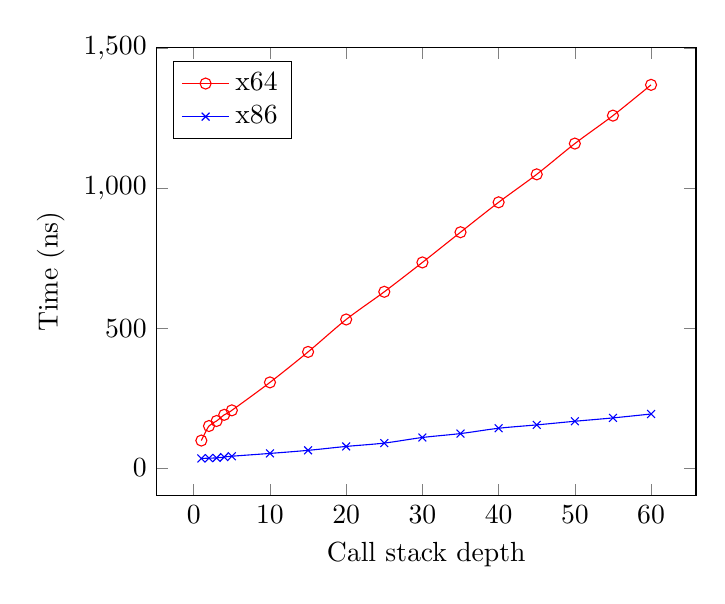
\begin{tikzpicture}
\begin{axis}[xlabel=Call stack depth,ylabel=Time (\si{\nano\second}), legend pos=north west]
\addplot[smooth, mark=o, red] plot coordinates {
(1, 98) (2, 150) (3, 168) (4, 190) (5, 206) (10, 306) (15, 415) (20, 531) (25, 630) (30, 735) (35, 843) (40, 950) (45, 1050) (50, 1160) (55, 1260) (60, 1370)
};
\addlegendentry{x64}
\addplot[smooth, mark=x, blue] plot coordinates {
(1, 34) (2, 35) (3, 36) (4, 39) (5, 42) (10, 52) (15, 63) (20, 77) (25, 89) (30, 109) (35, 123) (40, 142) (45, 154) (50, 167) (55, 179) (60, 193)
};
\addlegendentry{x86}
\end{axis}
\end{tikzpicture}
\caption{Plot of call stack capture times (see table~\ref{CallstackTimes}). Notice that the capture time grows linearly with requested capture depth}
\label{CallstackPlot}
\end{figure}

You can force call stack capture in the non-\texttt{S} postfixed macros by adding the \texttt{TRACY\_CALLSTACK} define, set to the desired call stack capture depth. This setting doesn't affect the explicit call stack macros.

The maximum call stack depth that can be retrieved is 62 frames. This is a restriction at the level of operating system.

\begin{bclogo}[
noborder=true,
couleur=black!5,
logo=\bcattention
]{Debugging symbols}
To have proper call stack information, the profiled application must be compiled with debugging symbols enabled. You can achieve that in the following way:

\begin{itemize}
\item On MSVC open the project properties and go to \emph{Linker\textrightarrow Debugging\textrightarrow Generate Debug Info}, where the \emph{Generate Debug Information} option should be selected.
\item On gcc or clang remember to specify the debugging information \texttt{-g} parameter during compilation and omit the strip symbols \texttt{-s} parameter. Link the executable with an additional option \texttt{-rdynamic} (or \texttt{-{}-export-dynamic}, if you are passing parameters directly to the linker).
\end{itemize}
\end{bclogo}

\subsection{Lua support}

To profile Lua code using Tracy, include the \texttt{tracy/TracyLua.hpp} header file in your Lua wrapper and execute \texttt{tracy::LuaRegister(lua\_State*)} function to add instrumentation support.

In the Lua code, add \texttt{tracy.ZoneBegin()} and \texttt{tracy.ZoneEnd()} calls to mark execution zones. You need to call the \texttt{ZoneEnd} method, because there is no automatic destruction of variables in Lua and we don't know when the garbage collection will be performed. \emph{Double check if you have included all return paths!}

Use \texttt{tracy.ZoneBeginN(name)} if you want to set a custom zone name\footnote{While technically this name doesn't need to be constant, like in the \texttt{ZoneScopedN} macro, it should be, as it is used to group the zones together. This grouping is then used to display various statistics in the profiler. You may still set the per-call name using the \texttt{tracy.ZoneName} method.}.

Use \texttt{tracy.ZoneText(text)} to set zone text.

Use \texttt{tracy.Message(text)} to send messages.

Use \texttt{tracy.ZoneName(text)} to set zone name on a per-call basis.

Lua instrumentation needs to perform additional work (including memory allocation) to store source location. This approximately doubles the data collection cost.

\subsubsection{Call stacks}

To collect Lua call stacks (see section~\ref{collectingcallstacks}), replace \texttt{tracy.ZoneBegin()} calls with \texttt{tracy.ZoneBeginS(depth)}, and \texttt{tracy.ZoneBeginN(name)} calls with \texttt{tracy.ZoneBeginNS(name, depth)}. Using the \texttt{TRACY\_CALLSTACK} macro automatically enables call stack collection in all zones.

Be aware that for Lua call stack retrieval to work, you need to be on a platform which supports collection of native call stacks.

Cost of performing Lua call stack capture is presented in table~\ref{CallstackTimesLua} and figure~\ref{CallstackPlotLua}. Lua call stacks include native call stacks, which have a capture cost of their own (table~\ref{CallstackTimes}) and the \texttt{depth} parameter is applied for both captures. The presented data was captured with full Lua stack depth, but only 13 frames were available on the native call stack. Hence, to explain the non-linearity of the graph you need to consider what was really measured:

\begin{displaymath}
\text{Cost}_{\text{total}}(\text{depth}) =
\begin{cases}
\text{Cost}_{\text{Lua}}(\text{depth}) + \text{Cost}_{\text{native}}(\text{depth}) & \text{when depth} \leq 13 \\
\text{Cost}_{\text{Lua}}(\text{depth}) + \text{Cost}_{\text{native}}(13) & \text{when depth} > 13
\end{cases}
\end{displaymath}

\begin{table}[h]
\centering
\begin{tabular}[h]{c|c}
\textbf{Depth} & \textbf{Time} \\ \hline
1 & 707 \si{\nano\second} \\
2 & 699 \si{\nano\second} \\
3 & 624 \si{\nano\second} \\
4 & 727 \si{\nano\second} \\
5 & 836 \si{\nano\second} \\
10 & 1.77 \si{\micro\second} \\
15 & 2.44 \si{\micro\second} \\
20 & 2.51 \si{\micro\second} \\
25 & 2.98 \si{\micro\second} \\
30 & 3.6 \si{\micro\second} \\
35 & 4.33 \si{\micro\second} \\
40 & 5.17 \si{\micro\second} \\
45 & 6.01 \si{\micro\second} \\
50 & 6.99 \si{\micro\second} \\
55 & 8.11 \si{\micro\second} \\
60 & 9.17 \si{\micro\second}
\end{tabular}
\caption{Median times of Lua zone capture with call stack (x64, 13 native frames)}
\label{CallstackTimesLua}
\end{table}

\begin{figure}[h]
\centering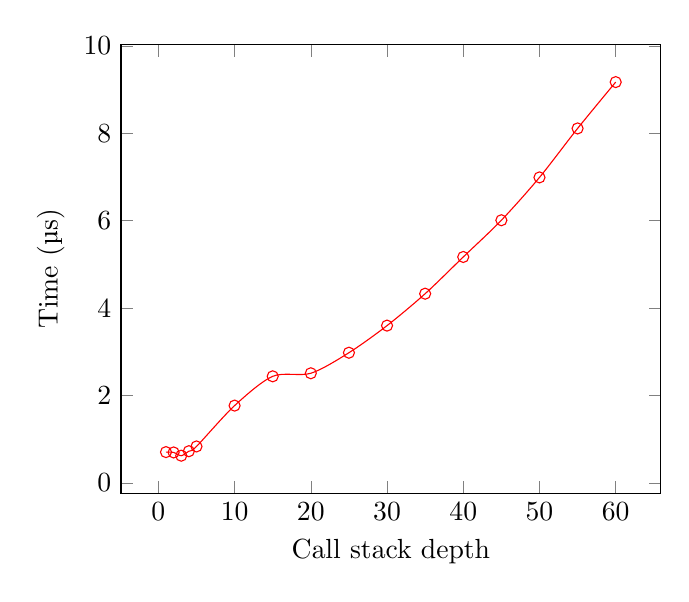
\begin{tikzpicture}
\begin{axis}[xlabel=Call stack depth,ylabel=Time (\si{\micro\second}), legend pos=north west]
\addplot[smooth, mark=o, red] plot coordinates {
(1, 0.707) (2, 0.699) (3, 0.624) (4, 0.727) (5, 0.836) (10, 1.770) (15, 2.440) (20, 2.510) (25, 2.980) (30, 3.600) (35, 4.330) (40, 5.170) (45, 6.010) (50, 6.990) (55, 8.110) (60, 9.170)
};
\end{axis}
\end{tikzpicture}
\caption{Plot of call Lua stack capture times (see table~\ref{CallstackTimesLua})}
\label{CallstackPlotLua}
\end{figure}

\subsubsection{Instrumentation cleanup}

Even if Tracy is disabled, you still have to pay the no-op function call cost. To prevent that you may want to use the \texttt{tracy::LuaRemove(char* script)} function, which will replace instrumentation calls with white-space. This function does nothing if profiler is enabled.

\subsection{C API}

In order to profile code written in C programming language, you will need to include the \texttt{tracy/TracyC.h} header file, which exposes the C API.

\begin{bclogo}[
noborder=true,
couleur=black!5,
logo=\bcbombe
]{Important}
Tracy is written in C++, so you will need to have a C++ compiler and link with C++ standard library, even if your program is strictly pure C.
\end{bclogo}

\begin{bclogo}[
noborder=true,
couleur=black!5,
logo=\bcattention
]{Caveats}
If you are using MSVC, you will need to disable the \emph{Edit And Continue} feature, for the C API to work\footnote{There's no such requirement for C++ API.}. To do so, open the project properties and go to \emph{C/C++\textrightarrow General\textrightarrow Debug Information Format} and make sure \emph{Program Database for Edit And Continue (/ZI)} is \emph{not} selected.
\end{bclogo}

\subsubsection{Zone markup}

The following macros mark the beginning of a zone:

\begin{itemize}
\item \texttt{TracyCZone(ctx, active)}
\item \texttt{TracyCZoneN(ctx, name, active)}
\item \texttt{TracyCZoneC(ctx, color, active)}
\item \texttt{TracyCZoneNC(ctx, name, color, active)}
\end{itemize}

Refer to sections~\ref{markingzones} and~\ref{multizone} for description of macro variants and parameters. The \texttt{ctx} parameter specifies the name of a data structure, which will hold internal zone data.

Unlike C++, there's no automatic destruction mechanism in C, so you will need to manually mark where the zone ends. To do so use the \texttt{TracyCZoneEnd(ctx)} macro.

Zone text and name may be set by using the \texttt{TracyCZoneText(ctx, txt, size)} and \texttt{TracyCZoneName(ctx, txt, size)} macros. Make sure you are following the zone stack rules, as described in section~\ref{multizone}!

\subsubsection{Zone validation}

Since all instrumentation using the C API has to be done by hand, it is possible to miss some code paths where a zone should be started or ended. Tracy will perform additional validation of instrumentation correctness to prevent bad profiling runs. Read section~\ref{instrumentationfailures} for more information.

The validation comes with a performance cost though, which you may not want to pay. If you are \emph{completely sure} that the instrumentation is not broken in any way, you may use the \texttt{TRACY\_NO\_VERIFY} macro, which will disable the validation code.

\section{Capturing the data}
\label{capturing}

After the client application has been instrumented, you will want to connect to it using a server.

\subsection{Command line}

You can capture a trace using a command line utility contained in the \texttt{capture} directory. To use it you will need to provide two parameters:

\begin{itemize}
\item \texttt{-a address} -- specifies the IP address (or a domain name) of the client application.
\item \texttt{-o output.tracy} -- the file name of the resulting trace.
\end{itemize}

If there is no client running at the given address, the server will wait until a connection can be made. During the capture the following information will be displayed:

\begin{verbatim}
% ./capture -a 127.0.0.1 -o trace
Connecting to 127.0.0.1...
Queue delay: 9 ns
Timer resolution: 6 ns
   1.90 Mbps | Ratio:  40.8% | Real:    4.67 Mbps | Mem: 77.57 MB
\end{verbatim}

The \emph{queue delay} and \emph{timer resolution} parameters are calibration results of timers used by the client. The next line is a status bar, which presents: network connection speed, connection compression ratio, the resulting uncompressed data rate and total memory usage of the utility.

You can disconnect from the client\footnote{\label{disconnect}The disconnect functionality is currently not implemented the right way and some data from the capture may be lost.} and save the captured trace by pressing \keys{\ctrl + C}.

\subsection{Interactive profiling}
\label{interactiveprofiling}

If you want to look at the profile data in real-time (or load a saved trace file), you can use the data analysis utility contained in the \texttt{profiler} directory. After starting the application, you will be greeted with a welcome dialog (figure~\ref{welcomedialog}), presenting a bunch of useful links (\faBook{}~\emph{User manual}, \faGlobeAmericas{}~\emph{Homepage} and \faVideo{}~\emph{Tutorial}).

The client \emph{address entry} field and the \faWifi{}~\emph{Connect} button are used to connect to a running client. You can use the connection history button~\faCaretDown{} to display a list of commonly used addresses, from which you can quickly select an address. You can remove entries from this list by hovering the \faMousePointer{}~mouse cursor over an entry and pressing the \keys{\del} button on the keyboard.

If you want to open a trace that you have stored on the disk, you can do so by pressing the \faFolderOpen{}~\emph{Open saved trace} button.

\begin{figure}[h]
\centering\begin{tikzpicture}
\draw (0, 0) rectangle (4.95, -2.9);
\draw[pattern=crosshatch dots] (0, 0) rectangle+(4.95, 0.3);
\draw[rounded corners=5pt] (0.1, -0.1) rectangle+(1.47, -0.5) node [midway] {\faBook};
\draw[rounded corners=5pt] (1.77, -0.1) rectangle+(1.47, -0.5) node [midway] {\faGlobeAmericas};
\draw[rounded corners=5pt] (3.37, -0.1) rectangle+(1.47, -0.5) node [midway] {\faVideo};

\draw (0.1, -0.9) rectangle+(4.1, -0.5) node [midway] {Address entry};
\draw[rounded corners=5pt] (4.33, -0.9) rectangle+(0.5, -0.5) node [midway] {\faCaretDown};
\draw[rounded corners=5pt] (0.1, -1.5) rectangle+(2, -0.5) node [midway] {\faWifi{}~Connect};
\draw[rounded corners=5pt] (0.1, -2.3) rectangle+(3.5, -0.5) node [midway] {\faFolderOpen{}~Open saved trace};
\end{tikzpicture}
\caption{Welcome dialog.}
\label{welcomedialog}
\end{figure}

Both connecting to a client and opening a saved trace will present you with the main profiler view, which you can use to analyze the data (see section~\ref{analyzingdata}).

If this is a real-time capture, you will also see the connection window (figure~\ref{connectioninfo}), with the capture status similar to the one displayed by the command line utility. This dialog also displays the connection speed graphed over time and the profiled application's current frames per second and frame time measurements. The circle displayed next to the bandwidth graph signals the connection status. If it's red, the connection is active. If it's gray, the client has disconnected.

You can use the \faSave{}~\emph{Save trace} button to save the current profile data to a file. Use the \faPlug{}~\emph{Stop} button to disconnect from the client (see footnote~\ref{disconnect}). The \faExclamationTriangle{}~\emph{Discard} button is used to discard current trace.

\begin{figure}[h]
\centering\begin{tikzpicture}
\draw (0, 0) rectangle (6.1, -2.7);
\draw[pattern=crosshatch dots] (0, 0) rectangle+(6.1, 0.3);
\draw[pattern=north east lines] (0.35, -0.35) circle(0.2);
\draw (0.7, -0.1) rectangle+(3.5, -0.5) node[midway] {Bandwidth graph};
\draw (4.3, -0.1) node[anchor=north west] {1.9 Mbps};
\draw (0.1, -0.6) node[anchor=north west] {Ratio 40.8\% \hspace{5pt} Real: 4.67 Mbps};
\draw (0.1, -1.1) node[anchor=north west] {Memory usage: 77.57 MB};
\draw (0.1, -1.6) node[anchor=north west] {FPS: 60 \hspace{5pt} Frame time: 16.7 ms};
\draw[rounded corners=5pt] (0.1, -2.1) rectangle+(2.2, -0.5) node [midway] {\faSave{}~Save trace};
\draw[rounded corners=5pt] (2.6, -2.1) rectangle+(1.3, -0.5) node [midway] {\faPlug{}~Stop};
\draw[rounded corners=5pt] (4.0, -2.1) rectangle+(2, -0.5) node [midway] {\faExclamationTriangle{}~Discard};
\end{tikzpicture}
\caption{Connection information window.}
\label{connectioninfo}
\end{figure}

\subsubsection{Automatic loading or connecting}

You can pass trace file name as an argument to the profiler application to open the capture, skipping the welcome dialog. You can also use the \texttt{-a address} argument to automatically connect to the given address.

\subsection{Connection speed}

Tracy will happily saturate a 1~Gbps network connection, as it can process up to 6~Gbps of uncompressed data. Note that at such data rates, the resulting capture will need to allocate about 1~GB of RAM per second.

\subsection{Memory usage}

The captured data is stored in RAM and only written to the disk, when the capture finishes. This can result in memory exhaustion when you are capturing massive amounts of profile data, or even in normal usage situations, when the capture is performed over a long stretch of time. The recommended usage pattern is to perform moderate instrumentation of the client code and limit capture time to the strict necessity.

In some cases it may be useful to perform an \emph{on-demand} capture, as described in section~\ref{ondemand}. In such case you will be able to profile only the interesting case (e.g.\ behavior during loading of a level in a game), ignoring all the unneeded data.

If you truly need to capture large traces, you have two options. Either buy more RAM, or use a large swap file on a fast disk drive\footnote{The operating system is able to manage memory paging much better than Tracy would be ever able to.}.

\subsection{Trace versioning}

Each new release of Tracy changes the internal format of trace files. While there is a backwards compatibility layer, allowing loading of traces created by previous versions of Tracy in new releases, it won't be there forever. You are thus advised to upgrade your traces using the utility contained in the \texttt{update} directory.

To use it, you will need to provide the input file and the output file. The program will print a short summary when it finishes:

\begin{verbatim}
% ./update old.tracy new.tracy
old.tracy (0.3.0) -> new.tracy (0.4.0)
\end{verbatim}

The new file contains the same data as the old one, but in the updated internal representation. Note that to perform an upgrade, whole trace needs to be loaded to memory.

\subsubsection{Archival mode}

The update utility supports optional higher level of data compression, enabled by passing the \texttt{-{}-hc} parameter. It can reduce the trace size by \numrange{15}{20}\%, at a considerable time cost ($\sim17\times$~increase of compression time).

Note that trace files (even the ones created in high compression mode) are optimized for fast decompression. You still will be able to squeeze the data using normal compression methods. For example, 7-zip can compress traces to about 25\% of their uncompressed\footnote{Compressed internally.} size.

\subsection{Instrumentation failures}
\label{instrumentationfailures}

In some cases your program may be incorrectly instrumented, for example you could have unbalanced zone begin and end events, or you could report a memory free event without first reporting a memory allocation event. When Tracy detects such misbehavior it immediately terminates connection with the client and displays an error message.

\section{Analyzing captured data}
\label{analyzingdata}

You have instrumented your application and you have captured a profiling trace. Now you want to look at the collected data. You can do this in the application contained in the \texttt{profiler} directory.

The workflow is identical, whether you are viewing a previously saved trace, or if you're performing a live capture, as described in section~\ref{interactiveprofiling}.

Note that loading a saved trace will display a progress window.

\subsection{Main profiler window}

The main profiler window is split into three sections, as seen on figure~\ref{mainwindow}: the control menu, the frame time graph and the timeline display.

\begin{figure}[h]
\centering\begin{tikzpicture}
\draw (0, 0) rectangle (15, -5.5);
\draw[pattern=crosshatch dots] (0, 0) rectangle+(15, 0.3);
\draw[rounded corners=5pt] (0.1, -0.1) rectangle+(0.5, -0.5) node [midway] {\faPowerOff};
\draw[rounded corners=5pt] (0.7, -0.1) rectangle+(1.8, -0.5) node [midway] {\faCog{} Options};
\draw[rounded corners=5pt] (2.6, -0.1) rectangle+(2.2, -0.5) node [midway] {\faTags{} Messages};
\draw[rounded corners=5pt] (4.9, -0.1) rectangle+(2.1, -0.5) node [midway] {\faSearch{} Find zone};
\draw[rounded corners=5pt] (7.1, -0.1) rectangle+(2, -0.5) node [midway] {\faSortAmountUp{} Statistics};
\draw[rounded corners=5pt] (9.2, -0.1) rectangle+(2, -0.5) node [midway] {\faMemory{} Memory};
\draw[rounded corners=5pt] (11.3, -0.1) rectangle+(2.1, -0.5) node [midway] {\faBalanceScale{} Compare};
\draw[rounded corners=5pt] (13.5, -0.1) rectangle+(1.3, -0.5) node [midway] {\faFingerprint{} Info};
\draw[rounded corners=5pt] (0.1, -0.7) rectangle+(0.4, -0.5) node [midway] {\faCaretLeft};
\draw (0.6, -0.7) node[anchor=north west] {Frames: 364};
\draw[rounded corners=5pt] (2.8, -0.7) rectangle+(0.4, -0.5) node [midway] {\faCaretRight};
\draw[rounded corners=5pt] (3.3, -0.7) rectangle+(0.5, -0.5) node [midway] {\faCaretDown};
\draw[rounded corners=5pt] (3.9, -0.7) rectangle+(0.5, -0.5) node [midway] {\faCrosshairs};
\draw (4.5, -0.7) node[anchor=north west] {\faEye~52.7 ms \hspace{5pt} \faDatabase~6.06 s};

\draw (0.1, -1.3) rectangle+(14.8, -1) node [midway] {Frame time graph};
\draw (0.1, -2.4) rectangle+(14.8, -3) node [midway] {Timeline view};
\end{tikzpicture}
\caption{Main profiler window. Note that the top line of buttons has been split into two rows in this manual.}
\label{mainwindow}
\end{figure}

\subsubsection{Control menu}
\label{controlmenu}

The control menu (top row of buttons) provides access to various features of the profiler. The buttons perform the following actions:

\begin{itemize}
\item \emph{\faPowerOff{} Close} -- This button unloads the current profiling trace and returns to the welcome menu, where another trace can be loaded. In live captures it is replaced by \emph{\faPause{}~Pause}, \emph{\faPlay{}~Resume} and \emph{\faSquare{}~Stopped} buttons.
\item \emph{\faPause{} Pause} -- While a live capture is in progress, the profiler will display the last three fully captured frames, so that you can see the current behavior of the program. Use this button\footnote{Or perform any action on the timeline view.} to stop the automatic updates of the timeline view (the capture will be still progressing).
\item \emph{\faPlay{} Resume} -- Use this button to resume following the most recent three frames in a live capture.
\item \emph{\faSquare{} Stopped} -- Inactive button used to indicate that the client application was terminated.
\item \emph{\faCog{} Options} -- Toggles the settings menu (section~\ref{options}).
\item \emph{\faTags{} Messages} -- Toggles the message log window (section~\ref{messages}), which displays custom messages sent by the client, as described in section~\ref{messagelog}.
\item \emph{\faSearch{} Find zone} -- This buttons toggles the find zone window, which allows inspection of zone behavior statistics (section~\ref{findzone}).
\item \emph{\faSortAmountUp{} Statistics} -- Toggles the statistics window, which displays zones sorted by their total time cost (section~\ref{statistics}).
\item \emph{\faMemory{} Memory} -- Various memory profiling options may be accessed here (section~\ref{memorywindow}).
\item \emph{\faBalanceScale{} Compare} -- Toggles the trace compare window, which allows you to see the performance difference between two profiling runs (section~\ref{compare}).
\item \emph{\faFingerprint{} Info} -- Show general information about the trace (section~\ref{traceinfo}).
\end{itemize}

The frame information block consists of four elements: the current frame set name along with the number of captured frames, the two navigational buttons \faCaretLeft{} and \faCaretRight{}, which allow you to focus the timeline view on the previous or next frame, and the frame set selection button \faCaretDown{}, which is used to switch to a another frame set\footnote{See section~\ref{framesets} for another way to change the active frame set.}. The \emph{\faCrosshairs{}~Go to frame} button allows zooming the timeline view on the specified frame. For more information about marking frames, see section~\ref{markingframes}.

The last two items show the \faEye{}~view time range and \faDatabase{}~time span of the whole capture.

\subsubsection{Frame time graph}

The graph of currently selected frame set (figure~\ref{frametime}) provides an outlook on the time spent in each frame, allowing you to see where the problematic frames are and to quickly navigate to them.

\begin{figure}[h]
\centering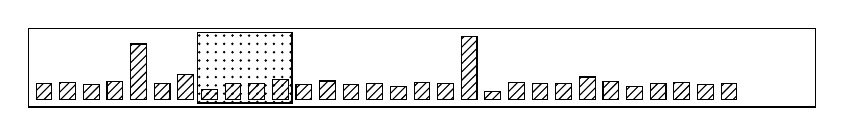
\begin{tikzpicture}
\draw (0, 0) rectangle (10, 1);

\draw[pattern=north east lines] (0.1, 0.1) rectangle+(0.2, 0.2);
\draw[pattern=north east lines] (0.4, 0.1) rectangle+(0.2, 0.21);
\draw[pattern=north east lines] (0.7, 0.1) rectangle+(0.2, 0.18);
\draw[pattern=north east lines] (1, 0.1) rectangle+(0.2, 0.22);
\draw[pattern=north east lines] (1.3, 0.1) rectangle+(0.2, 0.7);
\draw[pattern=north east lines] (1.6, 0.1) rectangle+(0.2, 0.2);
\draw[pattern=north east lines] (1.9, 0.1) rectangle+(0.2, 0.31);
\draw[pattern=north east lines] (2.2, 0.1) rectangle+(0.2, 0.12);
\draw[pattern=north east lines] (2.5, 0.1) rectangle+(0.2, 0.2);
\draw[pattern=north east lines] (2.8, 0.1) rectangle+(0.2, 0.2);
\draw[pattern=north east lines] (3.1, 0.1) rectangle+(0.2, 0.25);
\draw[pattern=north east lines] (3.4, 0.1) rectangle+(0.2, 0.19);
\draw[pattern=north east lines] (3.7, 0.1) rectangle+(0.2, 0.23);
\draw[pattern=north east lines] (4, 0.1) rectangle+(0.2, 0.19);
\draw[pattern=north east lines] (4.3, 0.1) rectangle+(0.2, 0.2);
\draw[pattern=north east lines] (4.6, 0.1) rectangle+(0.2, 0.16);
\draw[pattern=north east lines] (4.9, 0.1) rectangle+(0.2, 0.21);
\draw[pattern=north east lines] (5.2, 0.1) rectangle+(0.2, 0.2);
\draw[pattern=north east lines] (5.5, 0.1) rectangle+(0.2, 0.8);
\draw[pattern=north east lines] (5.8, 0.1) rectangle+(0.2, 0.1);
\draw[pattern=north east lines] (6.1, 0.1) rectangle+(0.2, 0.21);
\draw[pattern=north east lines] (6.4, 0.1) rectangle+(0.2, 0.2);
\draw[pattern=north east lines] (6.7, 0.1) rectangle+(0.2, 0.2);
\draw[pattern=north east lines] (7, 0.1) rectangle+(0.2, 0.28);
\draw[pattern=north east lines] (7.3, 0.1) rectangle+(0.2, 0.22);
\draw[pattern=north east lines] (7.6, 0.1) rectangle+(0.2, 0.16);
\draw[pattern=north east lines] (7.9, 0.1) rectangle+(0.2, 0.2);
\draw[pattern=north east lines] (8.2, 0.1) rectangle+(0.2, 0.21);
\draw[pattern=north east lines] (8.5, 0.1) rectangle+(0.2, 0.18);
\draw[pattern=north east lines] (8.8, 0.1) rectangle+(0.2, 0.2);

\draw[pattern=dots] (2.15, 0.05) rectangle+(1.2, 0.9);
\end{tikzpicture}
\caption{Frame time graph.}
\label{frametime}
\end{figure}

Each bar displayed on the graph represents an unique frame in the current frame set\footnote{Unless the view is zoomed out and multiple frames are merged into one column.}. The progress of time is in the right direction. The height of the bar indicates the time spent in frame, complemented with the color information:

\begin{itemize}
\item If the bar is \emph{blue}, then the frame met the \emph{best} time of 143 FPS, or 6.99 \si{\milli\second}\footnote{The actual target is 144 FPS, but one frame leeway is allowed to account for timing inaccuracies.}.
\item If the bar is \emph{green}, then the frame met the \emph{good} time of 59 FPS, or 16.94 \si{\milli\second}.
\item If the bar is \emph{yellow}, then the frame met the \emph{bad} time of 29 FPS, or 34.48 \si{\milli\second}.
\item If the bar is \emph{red}, then the frame didn't met any time limits.
\end{itemize}

The frames visible on the timeline are marked with a violet box drawn over them (presented as a dotted box on figure~\ref{frametime}).

Moving the \faMousePointer{} mouse cursor over the frames displayed on the graph will display tooltip with information about frame number, frame time, etc. Such tooltips are common for many UI elements in the profiler and won't be mentioned later in the manual.

The timeline view may be focused on the frames, by clicking or dragging the \LMB{} left mouse button on the graph. The graph may be scrolled left and right by dragging the \RMB{} right mouse button over the graph. The view may be zoomed in and out by using the \Scroll{} mouse scroll. If the view is zoomed out, so that multiple frames are merged into one column, the highest frame time will be used to represent the given column.

\subsubsection{Timeline view}

The timeline is the most important element of the profiler UI. All the captured data is displayed there, laid out on the horizontal axis, according to the flow of time. Where there was no profiling performed, the timeline is dimmed out. The view is split into three parts: the time scale, the frame sets and the combined zones, locks and plots display.

\subparagraph{Collapsed items}
\label{collapseditems}

Due to extreme differences in time scales, you will almost constantly see events that are too small to be displayed on the screen. Such events have preset minimum size (so they can be seen) and are marked with a zig-zag pattern, to indicate that you need to zoom-in to see more detail.

The zig-zag pattern can be seen applied to frame sets on figure~\ref{framesetsfig}, and to zones on figure~\ref{zoneslocks}.

\paragraph{Time scale}

The time scale is a quick aid in determining the relation between screen space and the time it represents (figure~\ref{timescale}).

\begin{figure}[h]
\centering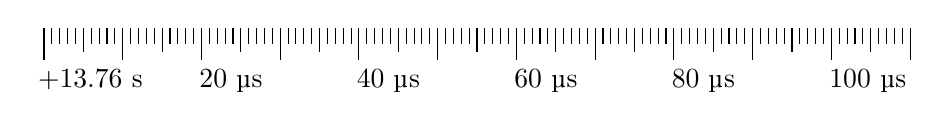
\begin{tikzpicture}
\foreach \x in {0,1,2,...,10} {
\draw (\x+0, 0) -- +(0, -0.4);
\draw (\x+0.1, 0) -- +(0, -0.2);
\draw (\x+0.2, 0) -- +(0, -0.2);
\draw (\x+0.3, 0) -- +(0, -0.2);
\draw (\x+0.4, 0) -- +(0, -0.2);
\draw (\x+0.5, 0) -- +(0, -0.3);
\draw (\x+0.6, 0) -- +(0, -0.2);
\draw (\x+0.7, 0) -- +(0, -0.2);
\draw (\x+0.8, 0) -- +(0, -0.2);
\draw (\x+0.9, 0) -- +(0, -0.2); }
\draw (11, 0) -- +(0, -0.4);

\draw (-0.2, -0.4) node[anchor=north west] {+13.76 s};
\draw (1.85, -0.4) node[anchor=north west] {20 \si{\micro\second}};
\draw (3.85, -0.4) node[anchor=north west] {40 \si{\micro\second}};
\draw (5.85, -0.4) node[anchor=north west] {60 \si{\micro\second}};
\draw (7.85, -0.4) node[anchor=north west] {80 \si{\micro\second}};
\draw (9.85, -0.4) node[anchor=north west] {100 \si{\micro\second}};
\end{tikzpicture}
\caption{Time scale.}
\label{timescale}
\end{figure}

The leftmost value on the scale represents the time at which the timeline starts. The rest of numbers label the notches on the scale, with some numbers omitted, if there's no space to display them.

\paragraph{Frame sets}
\label{framesets}

Frames from each frame set are displayed directly underneath the time scale. Each frame set occupies a separate row. The currently selected frame set is highlighted with bright colors, with the rest dimmed out.

\begin{figure}[h]
\centering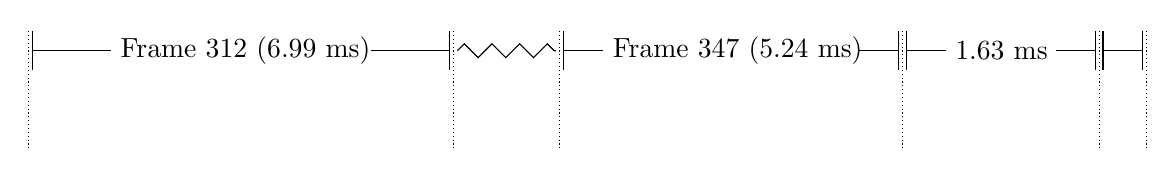
\begin{tikzpicture}
\draw[densely dotted] (-0.05, 0) -- +(0, -1.5);
\draw (0, 0) -- +(0, -0.5);
\draw (0, -0.25) -- +(1, 0) node[anchor=west] {Frame 312 (6.99 \si{\milli\second})};
\draw (4.3, -0.25) -- +(1, 0);
\draw (5.3, 0) -- +(0, -0.5);
\draw[densely dotted] (5.35, 0) -- +(0, -1.5);
\draw[decorate,decoration=zigzag] (5.4, -0.25) -- +(1.25, 0);
\draw[densely dotted] (6.7, 0) -- +(0, -1.5);
\draw (6.75, 0) -- +(0, -0.5);
\draw (6.75, -0.25) -- +(0.5, 0) node[anchor=west] {Frame 347 (5.24 \si{\milli\second})};
\draw (10.5, -0.25) -- +(0.5, 0);
\draw (11, 0) -- +(0, -0.5);
\draw[densely dotted] (11.05, 0) -- +(0, -1.5);
\draw (11.1, 0) -- +(0, -0.5);
\draw (11.1, -0.25) -- +(0.5, 0) node[anchor=west] {1.63 \si{\milli\second}};
\draw (13, -0.25) -- +(0.5, 0);
\draw (13.5, 0) -- +(0, -0.5);
\draw[densely dotted] (13.55, 0) -- +(0, -1.5);
\draw (13.6, 0) -- +(0, -0.5);
\draw (13.6, -0.25) -- +(0.5, 0);
\draw (14.1, 0) -- +(0, -0.5);
\draw[densely dotted] (14.15, 0) -- +(0, -1.5);
\end{tikzpicture}
\caption{Frames on the timeline.}
\label{framesetsfig}
\end{figure}

On figure~\ref{framesetsfig} we can see the fully described frames~312 and 347. The description consists of the frame name, which is \emph{Frame} for the default frame set (section~\ref{markingframes}) or the name you used for the secondary name set (section~\ref{secondaryframeset}), the frame number and the frame time. The frame~348 is too small to be fully displayed, so only the frame time is shown. The frame~349 is even smaller, with no space for any text. Moreover, frames~313~to~346 are too small to be displayed individually, so they are replaced with a zig-zag pattern, as described in section~\ref{collapseditems}.

You can also see that there are frame separators, projected down to the rest of the timeline view. Note that only the separators for the currently selected frame set are displayed. You can make a frame set active by clicking the \LMB{}~left mouse button on a frame set row you want to select (also see section~\ref{controlmenu}).

Clicking the \MMB{} middle mouse button on a frame will zoom the view to the extent of the frame.

\paragraph{Zones, locks and plots display}
\label{zoneslocksplots}

On this combined view you will find the zones with locks and their associated threads. The plots are graphed right below.

\begin{figure}[h]
\centering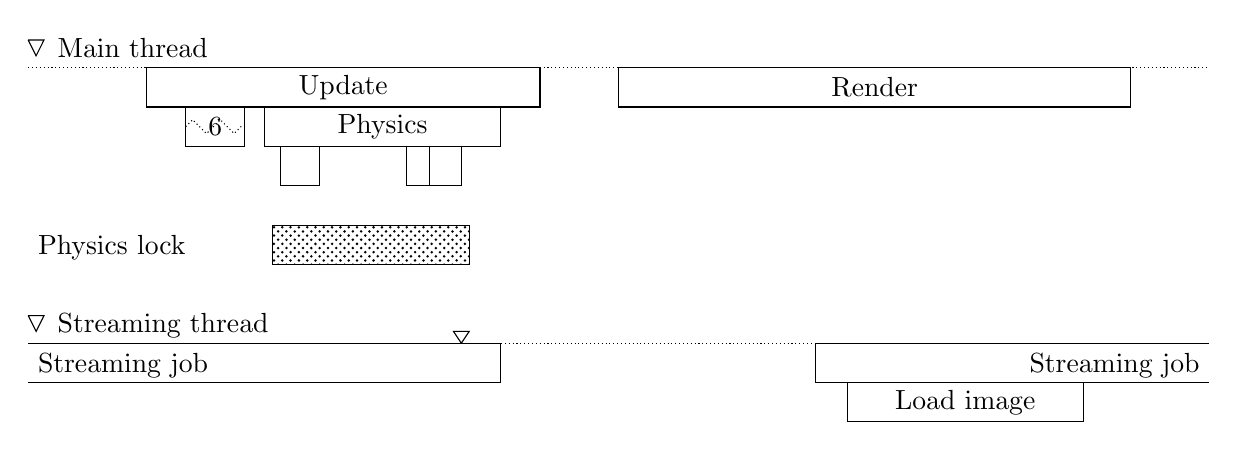
\begin{tikzpicture}
\draw(0, -0.15) -- (0.2, -0.15) -- (0.1, -0.35) -- (0, -0.15);
\draw(0.25, 0) node[anchor=north west] {Main thread};
\draw[densely dotted] (0, -0.5) -- +(15, 0);

\draw(1.5, -0.5) rectangle+(5, -0.5) node[midway] {Update};
\draw(2, -1) rectangle+(0.75, -0.5) node[midway] {6};
\draw[densely dotted, decorate,decoration=zigzag] (2, -1.25) -- +(0.75, 0 );
\draw(3, -1) rectangle+(3, -0.5) node[midway] {Physics};
\draw(3.2, -1.5) rectangle+(0.5, -0.5);
\draw(4.8, -1.5) rectangle+(0.3, -0.5);
\draw(5.1, -1.5) rectangle+(0.4, -0.5);

\draw(7.5, -0.5) rectangle+(6.5, -0.5) node[midway] {Render};

\draw(0, -2.5) node[anchor=north west] {Physics lock};
\draw[pattern=crosshatch dots] (3.1, -2.5) rectangle+(2.5, -0.5);

\draw(0, -3.65) -- (0.2, -3.65) -- (0.1, -3.85) -- (0, -3.65);
\draw(0.25, -3.5) node[anchor=north west] {Streaming thread};
\draw[densely dotted] (0, -4) -- +(15, 0);

\draw(0, -4) -- (6, -4) -- (6, -4.5) -- (0, -4.5);
\draw(5.5, -4) -- (5.4, -3.85) -- (5.6, -3.85) -- (5.5, -4);
\draw(0, -4) node[anchor=north west] {Streaming job};
\draw(15, -4) -- (10, -4) -- (10, -4.5) -- (15, -4.5);
\draw(15, -4) node[anchor=north east] {Streaming job};
\draw(10.4, -4.5) rectangle+(3, -0.5) node[midway] {Load image};
\end{tikzpicture}
\caption{Zones and locks display.}
\label{zoneslocks}
\end{figure}

The left hand side \emph{index area} of the timeline view displays various labels (threads, locks), which can be categorized in the following way:

\begin{itemize}
\item \emph{Light blue label} -- OpenGL/Vulkan context.
\item \emph{White label} -- A CPU thread. Will be replaced by a bright red label in a thread that has crashed (section~\ref{crashhandling}).
\item \emph{Light red label} -- Indicates a lock.
\item \emph{Yellow label} -- Plot.
\end{itemize}

Labels accompanied by the \faCaretDown{}~symbol can be collapsed out of the view, to reduce visual clutter. Hover the~\faMousePointer{}~mouse pointer over the label to display additional information. Click the \MMB{}~middle mouse button on a label to zoom the view to the extent of the label contents.

\subparagraph{Zones}

In an example on figure~\ref{zoneslocks} you can see that there are two threads: \emph{Main thread} and \emph{Streaming thread}\footnote{By clicking on a thread name you can temporarily disable display of the zones in this thread.}. We can see that the \emph{Main thread} has two root level zones visible: \emph{Update} and \emph{Render}. The \emph{Update} zone is split into further sub-zones, some of which are too small to be displayed at the current zoom level. This is indicated by drawing a zig-zag pattern over the merged zones box (section~\ref{collapseditems}), with the number of collapsed zones printed in place of zone name. We can also see that the \emph{Physics} zone acquires the \emph{Physics lock} mutex for the most of its run time.

Meanwhile the \emph{Streaming thread} is performing some \emph{Streaming jobs}. The first \emph{Streaming job} sent a message (section~\ref{messagelog}), which in addition to being listed in the message log is being indicated by the triangle over the thread separator. When there are multiple messages in one place, the triangle outline changes to a filled triangle.

At high zoom levels, the zones will be displayed with additional markers, as presented on figure~\ref{inaccuracy}. The red regions at the start and end of a zone indicate the cost associated with recording an event (\emph{Queue delay}). The error bars show the timer inaccuracy (\emph{Timer resolution}). Note that these markers are only \emph{approximations}, as there are many factors that can impact the true cost of capturing a zone, for example cache effects, or CPU frequency scaling, which is unaccounted for.

\begin{figure}[h]
\centering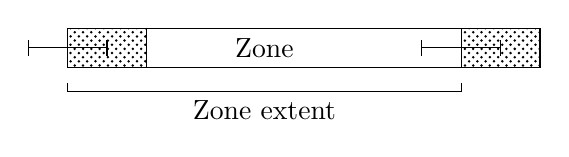
\begin{tikzpicture}
\draw(0, 0) rectangle+(5, 0.5) node [midway] {Zone};
\draw[pattern=crosshatch dots] (0, 0) rectangle+(1, 0.5);
\draw[pattern=crosshatch dots] (5, 0) rectangle+(1, 0.5);
\draw(-0.5, 0.35) -- (-0.5, 0.15);
\draw(0.5, 0.35) -- (0.5, 0.15);
\draw(-0.5, 0.25) -- (0.5, 0.25);
\draw(4.5, 0.35) -- (4.5, 0.15);
\draw(5.5, 0.35) -- (5.5, 0.15);
\draw(4.5, 0.25) -- (5.5, 0.25);
\draw(0, -0.2) -- (0, -0.3) -- (5, -0.3) -- (5, -0.2);
\draw(2.5, -0.3) node[anchor=north] {Zone extent};
\end{tikzpicture}
\caption{Approximation of timer inaccuracies and zone collection cost.}
\label{inaccuracy}
\end{figure}

The GPU zones are displayed just like CPU zones, with an OpenGL/Vulkan context in place of a thread name.

Hovering the \faMousePointer{} mouse pointer over a zone will highlight all other zones that have the same source location with a white outline. Clicking the \LMB{} left mouse button on a zone will open zone information window (section~\ref{zoneinfo}). Clicking the \MMB{} middle mouse button on a zone will zoom the view to the extent of the zone.

\subparagraph{Locks}

Mutual exclusion zones are displayed in each thread that tries to acquire them. There are three color-coded kinds of lock event regions that may be displayed. Note that when the timeline view is zoomed out, the contention regions are always displayed over the uncontented ones.

\begin{itemize}
\item \emph{Green region\footnote{This region type is disabled by default and needs to be enabled in options (section~\ref{options}).}} -- The lock is being held solely by one thread and no other thread tries to access it. In case of shared locks it is possible that multiple threads hold the read lock, but no thread requires a write lock.
\item \emph{Yellow region} -- The lock is being owned by this thread and some other thread also wants to acquire the lock.
\item \emph{Red region} -- The thread wants to acquire the lock, but is blocked by other thread, or threads in case of shared lock.
\end{itemize}

Hovering the \faMousePointer{}~mouse pointer over a lock timeline will highlight the lock in all threads to help reading the lock behavior. Hovering the \faMousePointer{}~mouse pointer over a lock event will display important information, for example a list of threads that are currently blocking, or which are blocked by the lock. Clicking the \LMB{}~left mouse button on a lock event or a lock label will open the lock information window, as described in section~\ref{lockwindow}. Clicking the \MMB{}~middle mouse button on a lock event will zoom the view to the extent of the event.

\subparagraph{Plots}
\label{plots}

The numerical data values (figure~\ref{plot}) are plotted right below the zones and locks. Note that the minimum and maximum values currently displayed on the plot are visible on the screen, along with the y range of the plot. The discrete data points are indicated with little rectangles. Multiple data points are indicated by a filled rectangle.

\begin{figure}[h]
\centering\begin{tikzpicture}
[dot/.style={rectangle,draw,scale=0.5}];
\draw(0, -0.15) -- (0.2, -0.15) -- (0.1, -0.35) -- (0, -0.15);
\draw(0.25, 0) node[anchor=north west] {Queue size (y-range: 463)};
\draw[densely dotted] (0, -0.5) -- +(15, 0);
\draw(0, -0.5) node[anchor=north west] {731};
\draw(0, -3) node[anchor=south west] {268};
\draw[densely dotted] (0, -3) -- +(15, 0);

\draw(0, -2) -- (1, -2.3) node[dot]{} -- (1.2, -3) node[dot]{} -- (6, -1.2) node[dot]{} -- (7, -0.5) node[dot]{} -- (9, -2) node[dot]{} -- (15, -2.5);
\end{tikzpicture}
\caption{Plot display.}
\label{plot}
\end{figure}

When memory profiling (section~\ref{memoryprofiling}) is enabled, Tracy will automatically generate a \emph{\faMemory{}~Memory usage} plot, which has extended capabilities. Hovering over a data point (memory allocation event) will visually display duration of the allocation. Clicking the \LMB{} left mouse button on the data point will open the memory allocation information window, which will display the duration of the allocation as long as the window is open.

Another plot that is automatically provided by Tracy is the \emph{\faTachometer*{}~CPU usage} plot. It is only available on some platforms and it represents the total system CPU usage percentage (it is not limited to the profiled application).

\subsubsection{Navigating the view}

Hovering the \faMousePointer{} mouse pointer over the timeline view will display a vertical line that can be used to visually line-up events in multiple threads. Dragging the \LMB{} left mouse button will display time measurement of the selected region.

The timeline view may be scrolled both vertically and horizontally by dragging the \RMB{} right mouse button. Note that only the zones, locks and plots scroll vertically, while the time scale and frame sets always stay in place.

You can zoom in and out the timeline view by using the \Scroll{} mouse scroll. You can select a range to which you want to zoom-in by dragging the \MMB{} middle mouse button. Dragging the \MMB{} middle mouse button while the \keys{\ctrl} key is pressed will zoom-out.

\subsection{Options menu}
\label{options}

In this window you can set various trace-related options. The timeline view might sometimes become overcrowded, in which case disabling display of some profiling events can increase readability.

\begin{itemize}
\item \emph{\faExpand{} Draw empty labels} -- By default threads that don't have anything to display at the current zoom level are hidden. Enabling this option will show them anyway.
\item \emph{\faEye{} Draw GPU zones} -- Allows disabling display of OpenGL/Vulkan zones. The \emph{GPU zones} drop-down allows disabling individual GPU contexts and setting CPU/GPU drift offsets (see section~\ref{gpuprofiling} for more information).
\item \emph{\faMicrochip{} Draw CPU zones} -- Determines whether CPU zones are displayed. The \emph{Namespaces} drop-down controls the display behavior of long zone names:
\begin{itemize}
\item \emph{Full} -- Zone names are always fully displayed (e.g.\ \texttt{std::sort}).
\item \emph{Shortened} -- If there's no space for full zone name, the namespaces will be shortened to one letter (e.g.\ \texttt{s::sort}).
\item \emph{None} -- If there's no space for full zone name, the namespaces will be omitted (e.g.\ \texttt{sort}).
\end{itemize}
\item \emph{\faLock{} Draw locks} -- Controls the display of locks. If the \emph{Only contended} option is selected, the non-blocking regions of locks won't be displayed (see section~\ref{zoneslocksplots}). The \emph{Locks} drop-down allows disabling display of locks on a per-lock basis. As a convenience, the list of locks is split into the single-threaded and multi-threaded categories. Clicking the \RMB{}~right mouse button on a lock label opens the lock information window (section~\ref{lockwindow}).
\item \emph{\faSignature{} Draw plots} -- Allows disabling display of plots. Individual plots can be disabled in the \emph{Plots} drop-down.
\item \emph{\faRandom{} Visible threads} -- Here you can disable display of selected threads.
\item \emph{\faImages{} Visible frame sets} -- Frame set display can be enabled or disabled here. Note that disabled frame sets are still available for selection in the frame set selection drop-down (section~\ref{controlmenu}), but are marked with a dimmed font.
\end{itemize}

Disabling display of some events is especially recommended when the profiler performance drops below acceptable levels for interactive usage.

\subsection{Messages window}
\label{messages}

In this window you can see all the messages that were sent by the client application, as described in section~\ref{messagelog}. The window is split into three columns: \emph{time}, \emph{thread} and \emph{message}. Hovering the \faMousePointer{} mouse cursor over a message will highlight it on the timeline view. Clicking the \LMB{} left mouse button on a message will center the timeline view on the selected message.

Message list can be filtered by the originating thread in the \emph{\faRandom{} Visible threads} drop-down.

\subsection{Statistics window}
\label{statistics}

Looking at the timeline view gives you a very localized outlook on things. Sometimes you want to look at the general overview of the program's behavior, for example you want to know which function takes the most of application's execution time. The statistics window provides you exactly that information.

Here you will find a multi-column display of captured zones, which contains: the zone \emph{name} and \emph{location}, \emph{total time} spent in the zone, the \emph{count} of zone executions and the \emph{mean time spent in the zone per call}. The view may be sorted according to the three displayed values.

By default the displayed times are inclusive, that is, they contain execution times of zone's children. If you want to view just the time spent in zone, you can enable the exclusive mode by selecting the \emph{\faClock{} Show self times} option.

Clicking the \LMB{} left mouse button on a zone will open the individual zone statistics view in the find zone window (section~\ref{findzone}).

\subsection{Find zone window}
\label{findzone}

The individual behavior of zones may be influenced by many factors, like CPU cache effects, access times amortized by the disk cache, thread context switching, etc. Sometimes the execution time depends on the internal data structures and their response to different inputs. In other words, it is hard to determine the true performance characteristics by looking at any single zone.

Tracy gives you the ability to display an execution time histogram of all occurrences of a zone. On this view you can see how the function behaves in general, ignoring the outliers. You can inspect how various data inputs influence the execution time and you can filter the data to eventually drill down to the individual zone calls, so that you can see the environment in which they were called.

You start by entering a search query, which will be matched against known zone names (see section~\ref{markingzones} for information on the grouping of zone names). If the search found some results, you will be presented with a list of zones in the \emph{matched source locations} drop-down. The selected zone's graph is displayed on the \emph{histogram} drop-down and also the matching zones are highlighted on the timeline view. Clicking the \RMB{} right mouse button on the source file location will open the source file view window (if applicable, see section~\ref{sourceview}).

An example histogram is presented on figure~\ref{findzonehistogram}. Here you can see that the majority of zone calls (by count) are clustered in the 300~\si{\nano\second} group, closely followed by the 10~\si{\micro\second} cluster. There are some outliers at the 1~and~10~\si{\milli\second} marks, which can be ignored on most occasions, as these are single occurrences.

\begin{figure}[h]
\centering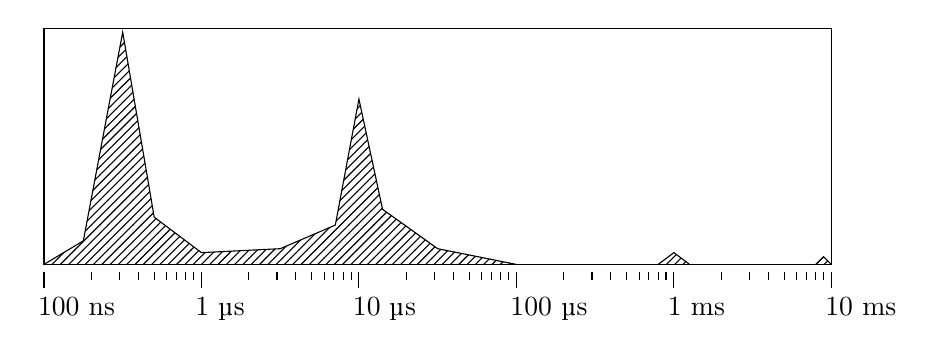
\begin{tikzpicture}
\draw(0, 0) rectangle+(10, 3);
\foreach \x in {0,2,4,6,8} {
\draw (\x+0, -0.1) -- +(0, -0.2);
\draw (\x+0.6, -0.1) -- +(0, -0.1);
\draw (\x+0.96, -0.1) -- +(0, -0.1);
\draw (\x+1.2, -0.1) -- +(0, -0.1);
\draw (\x+1.4, -0.1) -- +(0, -0.1);
\draw (\x+1.56, -0.1) -- +(0, -0.1);
\draw (\x+1.68, -0.1) -- +(0, -0.1);
\draw (\x+1.8, -0.1) -- +(0, -0.1);
\draw (\x+1.9, -0.1) -- +(0, -0.1); }
\draw (10, -0.1) -- +(0, -0.2);

\draw (-0.2, -0.3) node[anchor=north west] {100 \si{\nano\second}};
\draw (1.8, -0.3) node[anchor=north west] {1 \si{\micro\second}};
\draw (3.8, -0.3) node[anchor=north west] {10 \si{\micro\second}};
\draw (5.8, -0.3) node[anchor=north west] {100 \si{\micro\second}};
\draw (7.8, -0.3) node[anchor=north west] {1 \si{\milli\second}};
\draw (9.8, -0.3) node[anchor=north west] {10 \si{\milli\second}};

\draw[pattern=north east lines] (0,0) -- (0.5, 0.3) -- (1, 2.95) -- (1.4, 0.6) -- (2, 0.15) -- (3, 0.2) -- (3.7, 0.5) -- (4, 2.1) -- (4.3, 0.7) -- (5, 0.2) -- (6, 0);
\draw[pattern=north east lines] (7.8,0) -- (8, 0.15) -- (8.2, 0);
\draw[pattern=north east lines] (9.8,0) -- (9.9, 0.1) -- (10, 0);
\end{tikzpicture}
\caption{Zone execution time histogram.}
\label{findzonehistogram}
\end{figure}

The histogram is accompanied by various data statistics about displayed data, for example the \emph{total time} of the displayed samples, or the \emph{maximum number of counts} in histogram bins. There are four options that control how the data is presented:

\begin{itemize}
\item \emph{Log values} -- Switches between linear and logarithmic scale on the y~axis of the graph, representing the call counts\footnote{Or time, if the \emph{cumulate time} option is enabled.}.
\item \emph{Log time} -- Switches between linear and logarithmic scale on the x~axis of the graph, representing the time bins.
\item \emph{Cumulate time} -- Changes how the histogram bin values are calculated. By default the vertical bars on the graph represent the \emph{call counts} of zones that fit in the given time bin. If this option is enabled, the bars represent the \emph{time spent} in the zones. For example, on graph presented on figure~\ref{findzonehistogram} the 10~\si{\micro\second} cluster is the dominating one, if we look at the time spent in zone, even if the 300~\si{\nano\second} cluster has greater number of call counts.
\item \emph{Self time} -- Removes children time from the analysed zones, which results in displaying only the time spent in the zone itself (or in non-instrumented function calls).
\end{itemize}

You can drag the \LMB{} left mouse button over the histogram to select a time range that you want to closely look at. This will display the data in the histogram info section and it will also filter zones displayed in the \emph{found zones} section. This is quite useful, if you want to actually look at the outliers, i.e.\ where did they originate from, what the program was doing at the moment, etc\footnote{More often than not you will find out, that the application was just starting, or an access to a cold file was required and there's not much you can do to optimize that particular case.}. You can reset the selection range by pressing the \RMB{} right mouse button on the histogram.

The \emph{found zones} section displays the individual zones grouped according to the following criteria:

\begin{itemize}
\item \emph{Thread} -- In this mode you can see which threads were executing the zone.
\item \emph{User text} -- Splits the zones according to the custom user text (see section~\ref{markingzones}).
\item \emph{Call stacks} -- Zones are grouped by the originating call stack (see section~\ref{collectingcallstacks}). Note that two call stacks may sometimes appear identical, even if they not, due to an easy to overlook difference in the source line numbers.
\end{itemize}

Each group may be sorted according to the \emph{order} in which it appeared, the call \emph{count}, the total \emph{time} spent in the group, or the \emph{mean time per call}. Expanding the group view will display individual occurrences of the zone, which can be sorted by application's time, execution time or zone's name. Clicking the \LMB{} left mouse button on a zone will open the zone information window (section~\ref{zoneinfo}). Clicking the \MMB{} middle mouse button on a zone will zoom the timeline view to the zone's extent.

Clicking the \LMB{} left mouse button on group name will highlight the group time data on the histogram (figure~\ref{findzonehistogramgroup}). This function provides a quick insight about the impact of the originating thread, or input data on the zone performance. Clicking the \RMB{} right mouse button on the group names area will reset the group selection.

\begin{figure}[h]
\centering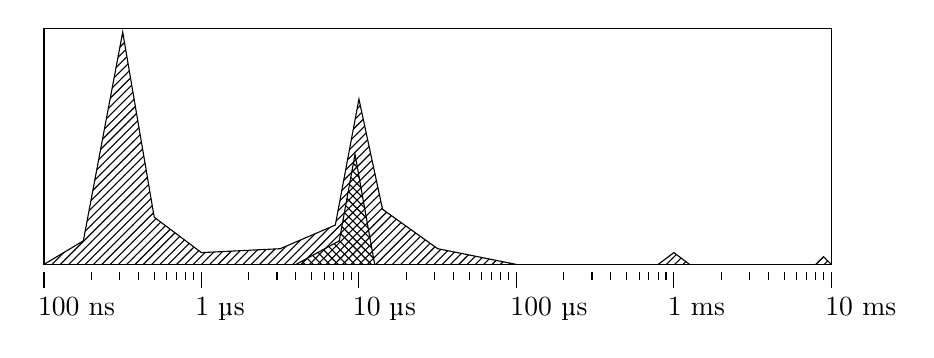
\begin{tikzpicture}
\draw(0, 0) rectangle+(10, 3);
\foreach \x in {0,2,4,6,8} {
\draw (\x+0, -0.1) -- +(0, -0.2);
\draw (\x+0.6, -0.1) -- +(0, -0.1);
\draw (\x+0.96, -0.1) -- +(0, -0.1);
\draw (\x+1.2, -0.1) -- +(0, -0.1);
\draw (\x+1.4, -0.1) -- +(0, -0.1);
\draw (\x+1.56, -0.1) -- +(0, -0.1);
\draw (\x+1.68, -0.1) -- +(0, -0.1);
\draw (\x+1.8, -0.1) -- +(0, -0.1);
\draw (\x+1.9, -0.1) -- +(0, -0.1); }
\draw (10, -0.1) -- +(0, -0.2);

\draw (-0.2, -0.3) node[anchor=north west] {100 \si{\nano\second}};
\draw (1.8, -0.3) node[anchor=north west] {1 \si{\micro\second}};
\draw (3.8, -0.3) node[anchor=north west] {10 \si{\micro\second}};
\draw (5.8, -0.3) node[anchor=north west] {100 \si{\micro\second}};
\draw (7.8, -0.3) node[anchor=north west] {1 \si{\milli\second}};
\draw (9.8, -0.3) node[anchor=north west] {10 \si{\milli\second}};

\draw[pattern=north east lines] (0,0) -- (0.5, 0.3) -- (1, 2.95) -- (1.4, 0.6) -- (2, 0.15) -- (3, 0.2) -- (3.7, 0.5) -- (4, 2.1) -- (4.3, 0.7) -- (5, 0.2) -- (6, 0);
\draw[pattern=north east lines] (7.8,0) -- (8, 0.15) -- (8.2, 0);
\draw[pattern=north east lines] (9.8,0) -- (9.9, 0.1) -- (10, 0);

\draw[pattern=north west lines] (3.2, 0) -- (3.75, 0.3) -- (3.95, 1.4) -- (4.2, 0);
\end{tikzpicture}
\caption{Zone execution time histogram with a group highlighted.}
\label{findzonehistogramgroup}
\end{figure}

The call stack grouping mode has a different way of listing groups. Here only one group is displayed at any time, due to need to display the call stack frames. You can switch between call stack groups by using the~\faCaretLeft{}~and~\faCaretRight{} buttons. The group can be selected by clicking on the~\emph{\faCheck{}~Select} button (to reset the group selection use the~\RMB{}~right mouse button, as usual). You can open the call stack window (section~\ref{callstackwindow}) by pressing the~\emph{\faAlignJustify{}~Call~stack} button.

The average and median zone times are displayed on the histogram as a red (average) and blue (median) vertical bars. When a group is selected, additional bars will indicate the average group time (orange) and median group time (green). You can disable drawing of either set of markers by clicking on the check-box next to the color legend.

\begin{bclogo}[
noborder=true,
couleur=black!5,
logo=\bclampe
]{Keyboard shortcut}
You may press \keys{\ctrl + F} to open or focus the find zone window and set the keyboard input on the search box.
\end{bclogo}

\subsection{Compare traces window}
\label{compare}

Comparing the performance impact of the optimization work is not an easy thing to do. Benchmarking is often inconclusive, if even possible, in case of interactive applications, where the benchmarked function might not have a visible impact on frame render time. Doing isolated micro-benchmarks loses the execution environment of the application, in which many different functions compete for limited system resources.

Tracy solves this problem by providing a compare traces functionality, very similar to the find zone window, described in section~\ref{findzone}.

You would begin your work by recording a reference trace that represents the usual behavior of the program. Then, after the optimization of the code is completed, you record another trace, doing roughly what you did for the reference one. Having the optimized trace open you select the \emph{\faFolderOpen{}~Open second trace} option in the compare traces window and load the reference trace.

Now things start to get familiar. You search for a zone, similarly like in the find zone window, choose the one you want in the \emph{matched source locations} drop-down, and then you look at the histogram. This time there are two overlaid graphs, one representing the current trace, and the second one representing the external (reference) trace (figure~\ref{comparehistogram}). You can easily see how the performance characteristics of the zone were affected by your modifications.

\begin{figure}[h]
\centering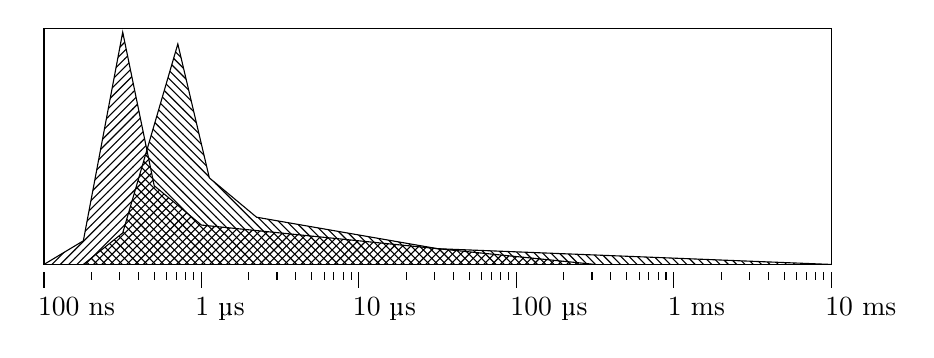
\begin{tikzpicture}
\draw(0, 0) rectangle+(10, 3);
\foreach \x in {0,2,4,6,8} {
\draw (\x+0, -0.1) -- +(0, -0.2);
\draw (\x+0.6, -0.1) -- +(0, -0.1);
\draw (\x+0.96, -0.1) -- +(0, -0.1);
\draw (\x+1.2, -0.1) -- +(0, -0.1);
\draw (\x+1.4, -0.1) -- +(0, -0.1);
\draw (\x+1.56, -0.1) -- +(0, -0.1);
\draw (\x+1.68, -0.1) -- +(0, -0.1);
\draw (\x+1.8, -0.1) -- +(0, -0.1);
\draw (\x+1.9, -0.1) -- +(0, -0.1); }
\draw (10, -0.1) -- +(0, -0.2);

\draw (-0.2, -0.3) node[anchor=north west] {100 \si{\nano\second}};
\draw (1.8, -0.3) node[anchor=north west] {1 \si{\micro\second}};
\draw (3.8, -0.3) node[anchor=north west] {10 \si{\micro\second}};
\draw (5.8, -0.3) node[anchor=north west] {100 \si{\micro\second}};
\draw (7.8, -0.3) node[anchor=north west] {1 \si{\milli\second}};
\draw (9.8, -0.3) node[anchor=north west] {10 \si{\milli\second}};

\draw[pattern=north east lines] (0,0) -- (0.5, 0.3) -- (1, 2.95) -- (1.4, 1) -- (2, 0.5) -- (7, 0);
\draw[pattern=north west lines] (0.5,0) -- (1, 0.4) -- (1.7, 2.8) -- (2.1, 1.1) -- (2.7, 0.6) -- (5, 0.2) -- (10, 0);
\end{tikzpicture}
\caption{Compare traces histogram.}
\label{comparehistogram}
\end{figure}

Note that the traces are color and symbol coded. The current trace is marked by a yellow \faLemon{} symbol, and the external one is marked by a red \faGem{} symbol.

It may be difficult, if not impossible, to perform identical runs of a program. This means that the number of collected zones may differ in both traces, which would influence the displayed results. To fix this problem enable the \emph{Normalize values} option, which will adjust the displayed results as-if both traces had the same number of recorded zones.

\subsection{Memory window}
\label{memorywindow}

The data gathered by profiling memory usage (section~\ref{memoryprofiling}) can be viewed in the memory window. The top row contains statistics, such as \emph{total allocations} count, number of \emph{active allocations}, current \emph{memory usage} and process \emph{memory span}\footnote{Memory span describes the address space consumed by the program. It is calculated as a difference between the maximum and minimum observed in-use memory address.}.

The lists of captured memory allocations are displayed in a common multi-column format thorough the profiler. The first column specifies the memory address of an allocation, or an address and an offset, if the address is not at the start of the allocation. Clicking the \LMB{} left mouse button on an address will open the memory allocation information window\footnote{While the allocation information window is opened, the address will be highlighted on the list.} (see section~\ref{memallocinfo}). Clicking the \MMB{}~middle mouse button on an address will zoom the timeline view to memory allocation's range. The next column contains the allocation size.

The allocation's timing data is contained in two columns: \emph{appeared at} and \emph{duration}. Clicking the \LMB{}~left mouse button on the first one will center the timeline view at the beginning of allocation, and likewise, clicking on the second one will center the timeline view at the end of allocation. Note that allocations that have not yet been freed will have their duration displayed in green color.

The memory event location in the code is displayed in the last four columns. The \emph{thread} column contains the thread where the allocation was made and freed (if applicable), or an \emph{alloc / free} pair of threads, if it was allocated in one thread and freed in another. The \emph{zone alloc} contains the zone in which the allocation was performed\footnote{The actual allocation is typically a couple functions deeper in the call stack.}, or \texttt{-} if there was no active zone in the given thread at the time of allocation. Clicking the \LMB{}~left mouse button on the zone name will open the zone information window (section~\ref{zoneinfo}). Similarly, the \emph{zone free} column displays the zone which freed the allocation, which may be colored yellow, if it is the same exact zone that did the allocation. Alternatively, if the zone has not yet been freed, a green \emph{active} text is displayed. The last column contains the \emph{alloc} and \emph{free} call stack buttons, or their placeholders, if no call stack is available (see section~\ref{collectingcallstacks} for more information). Clicking on either of the buttons will open the call stack window (section~\ref{callstackwindow}). Note that the call stack buttons that match the information window will be highlighted.

The memory window is split into the following sections:

\subsubsection{Allocations}

The \emph{\faAt{} Allocations} pane allows you to search for the specified address usage during the whole life-time of the program. All recorded memory allocations that match the query will be displayed on a list.

\subsubsection{Active allocations}

The \emph{\faHeartbeat{} Active allocations} pane displays a list of currently active memory allocations and their total memory usage. Here you can see where exactly your program did allocate memory it is currently using. If the application has already exited, this becomes a list of leaked memory.

\subsubsection{Memory map}

On the \emph{\faMap{} Memory map} pane you can see the graphical representation of your program's address space. Active allocations are displayed as green lines, while the freed memory is marked as red lines. The brightness of the color indicates how much time has passed since the last memory event at the given location -- the most recent events are the most vibrant.

This view may be helpful in assessing the general memory behavior of the application, or in debugging the problems resulting from address space fragmentation.

\subsubsection{Bottom-up call stack tree}
\label{callstacktree}

The \emph{\faAlignJustify{}~Bottom-up call stack tree} pane is only available, if the memory events were collecting the call stack data (section~\ref{collectingcallstacks}). In this view you are presented with a tree of memory allocations, starting at the call stack entry point and going up to the allocation's pinpointed place. Each level of the tree is sorted according to the number of bytes allocated in given branch.

Each tree node consists of three elements: the function name, the source file location and the memory allocation data. The memory allocation data is either yellow \emph{inclusive} events count (allocations performed by children), or the cyan \emph{exclusive} events count (allocations that took place in the node)\footnote{Due to the way call stacks work there is no possibility for an entry to have both inclusive and exclusive counts, in a properly instrumented program.}. There are two values that are counted: total memory size and number of allocations.

The \emph{Group by function name} option controls how tree nodes are grouped. If it is disabled, then the grouping is performed at a machine instruction level granularity. This may result in very verbose output, but the displayed source locations are precise. To make the tree more readable you may opt to perform grouping at the function name level, which will result in less valid source file locations, as multiple entries are collapsed into one.

Clicking the \RMB{}~right mouse button on the function name will open allocations list window (see section \ref{alloclist}), which list all the allocations included at the current call stack tree level. Clicking the \RMB{}~right mouse button on the source file location will open the source file view window (if applicable, see section~\ref{sourceview}).

Some function names may be too long to be properly displayed, with the events count data at the end. In such cases, you may press the \emph{control} button, which will display events count tooltip.

\subsubsection{Top-down call stack tree}

This pane is identical in functionality to the \emph{Bottom-up call stack tree}, but the call stack order is reversed when the tree is built. This means that the tree starts at the memory allocation functions and goes down to the call stack entry point.

\subsubsection{Looking back at the memory history}

By default the memory window displays the memory data at the current point of program execution. It is however possible to view the historical data by enabling the \emph{\faHistory{}~Restrict time} option. This will draw a vertical violet line on the timeline view, which will act as a terminator for memory events. The memory window will use only the events lying on the left side of the terminator line (in the past), ignoring everything that's on the right side.

\subsection{Allocations list window}
\label{alloclist}

This window displays the list of allocations included at the selected call stack tree level (see section~\ref{memorywindow} and \ref{callstacktree}).

\subsection{Memory allocation information window}
\label{memallocinfo}

The information about the selected memory allocation is displayed in this window. It lists the allocation's address and size, along with the time, thread and zone data of the allocation and free events. Clicking the \emph{\faMicroscope{}~Zoom to allocation} button will zoom the timeline view to the allocation's extent.

\subsection{Trace information window}
\label{traceinfo}

This window contains various bits of information about profiler and the current trace. For example, you can see the profiler memory usage, the number of captured zones, lock event, plot points, memory allocations, etc. There's also a section containing the selected frame set timing statistics and histogram\footnote{See section~\ref{findzone} for a description of the histogram. Note that there are subtle differences in the available functionality.}.

In this window you can view the information about the machine on which the profiled application was running. This includes the operating system, the used compiler, CPU name, amount of total available RAM, etc.

Here you will also be able to see the tombstone generated during an application's crash (section~\ref{crashhandling}). It provides you with information about the thread that has crashed, the crash reason and the crash call stack (section~\ref{callstackwindow}).

\subsection{Zone information window}
\label{zoneinfo}

The zone information window displays detailed information about a single zone. There can be only one zone information window open at any time. While the window is open the zone will be highlighted on the timeline view with a green outline. The following data is presented:

\begin{itemize}
\item Basic source location information: function name, source file location and the thread name.
\item Timing information.
\item Memory events list, both summarized and a list of individual allocation/free events (see section~\ref{memorywindow} for more information on the memory events list).
\item List of messages that were logged in the zone's scope (including its children).
\item Zone trace, taking into account the zone tree and call stack information (section~\ref{collectingcallstacks}), trying to reconstruct a combined zone + call stack trace\footnote{Reconstruction is only possible, if all zones have full call stack capture data available. In case where that's not available, an \emph{unknown frames} entry will be present.}. Captured zones are displayed as normal text, while functions that were not instrumented are dimmed. Hovering the \faMousePointer{}~mouse pointer over a zone will highlight it on the timeline view with a red outline. Clicking the \LMB{}~left mouse button on a zone will switch the zone info window to that zone. Clicking the \MMB{}~middle mouse button on a zone will zoom the timeline view to the zone's extent. Clicking the \RMB{}~right mouse button on a source file location will open the source file view window (if applicable, see section~\ref{sourceview}).
\item Child zones list, showing how the current zone's execution time was used. Zones on this list can be grouped according to their source location. Each group can be expanded to show individual entries. All the controls from the zone trace are also available here.
\end{itemize}

The zone information window has the following controls available:

\begin{itemize}
\item \emph{\faMicroscope{} Zoom to zone} -- Zooms the timeline view to the zone's extent.
\item \emph{\faArrowUp{} Go to parent} -- Switches the zone information window to display current zone's parent zone (if available).
\item \emph{\faChartBar{} Statistics} -- Displays the zone general performance characteristics in the find zone window (section~\ref{findzone}).
\item \emph{\faAlignJustify{} Call stack} -- Views the current zone's call stack in the call stack window (section~\ref{callstackwindow}). The button will be highlighted, if the call stack window shows the zone's call stack. Only available if zone had captured call stack data (section~\ref{collectingcallstacks}).
\item \emph{\faFile*{} Source} -- Display source file view window with the zone source code (only available if applicable, see section~\ref{sourceview}). Button will be highlighted, if the source file is being currently displayed (but the focused source line might be different).
\item \emph{\faArrowLeft{} Go back} -- Returns to the previously viewed zone. The viewing history is lost when the zone information window is closed, or when the type of displayed zone changes (from CPU to GPU or vice versa).
\end{itemize}

\subsection{Call stack window}
\label{callstackwindow}

This window shows the frames contained in the selected call stack. Each frame is described by the function name and source file location. Clicking the \LMB{}~left mouse button on either the function name of source file location will copy the name to the clipboard. Clicking the \RMB{}~right mouse button on the source file location will open the source file view window (if applicable, see section~\ref{sourceview}).

A single stack frame may have multiple function call places associated with it. This happens in case of inlined function calls. Such entries will be displayed in the call stack window, with \emph{inline} in place of frame number.

Sometimes it may be more useful to have just the function address, instead of the source file location\footnote{It can pinpoint the exact assembly instruction which caused the crash.}. This can be achieved by selecting the \emph{\faAt{}~Show frame addresses} option.

\subsubsection{Reading call stacks}

You need to take special care when reading call stacks. Contrary to their name, call stacks do not show \emph{function call stacks}, but rather \emph{function return stacks}. This might be a bit confusing at first, but this is how programs do work. Consider the following source code:

\begin{lstlisting}
int main()
{
    auto app = std::make_unique<Application>();
    app->Run();
    app.reset();
}
\end{lstlisting}

Let's say you are looking at the call stack of some function called within \texttt{Application::Run}. This is the result you might get:

\begin{lstlisting}
0. @\ldots@
1. @\ldots@
2. Application::Run
3. std::unique_ptr<Application>::reset
4. main
\end{lstlisting}

At the first glance it may look like \texttt{unique\_ptr::reset} was the \emph{call site} of the \texttt{Application::Run}, which would make no sense, but this is not the case here. When you remember these are the \emph{function return points}, it becomes much more clear what is happening. As an optimization, \texttt{Application::Run} is returning directly into \texttt{unique\_ptr::reset}, skipping the return to \texttt{main} and an unnecessary \texttt{reset} function call.

\subsection{Source file view window}
\label{sourceview}

In this window you can view the source code of the profiled application, to take a quick glance at the context of the function behavior you are analyzing.

\begin{bclogo}[
noborder=true,
couleur=black!5,
logo=\bcbombe
]{Important}
Source file view works on the local files you have on your disk. The traces themselves do not contain any source code! This has the following implications:

\begin{itemize}
\item The source files can only be viewed, if the source file location recorded in the trace matches the files you have on your disk.
\item \textbf{The displayed source files might not reflect the code that was profiled!} It is up to you to verify that you don't have a modified version of the code, with regards to the trace.
\end{itemize}
\end{bclogo}

\subsection{Lock information window}
\label{lockwindow}

This window presents information and statistics about a lock. The lock events count represents the total number collected of wait, obtain and release events. The announce, termination and lock lifetime measure the time from the lockable construction until destruction.

\newpage
\appendix
\appendixpage

\section{License}

\verbatiminput{../LICENSE.}

\section{List of contributors}

\verbatiminput{../AUTHORS.}

\section{Inventory of external libraries}

The following libraries are included with and used by the Tracy Profiler:

\begin{itemize}
\item 3-clause BSD license
\begin{itemize}
\item getopt\_port -- \url{https://github.com/kimgr/getopt\_port}
\item libbacktrace -- \url{https://github.com/ianlancetaylor/libbacktrace}
\end{itemize}

\item 2-clause BSD license
\begin{itemize}
\item concurrentqueue -- \url{https://github.com/cameron314/concurrentqueue}
\item LZ4 -- \url{https://github.com/lz4/lz4}
\end{itemize}

\item Public domain
\begin{itemize}
\item rpmalloc -- \url{https://github.com/rampantpixels/rpmalloc}
\item gl3w -- \url{https://github.com/skaslev/gl3w}
\end{itemize}

\item zlib license
\begin{itemize}
\item benaphore -- \url{https://github.com/preshing/cpp11-on-multicore}
\item Native File Dialog -- \url{https://github.com/mlabbe/nativefiledialog}
\item GLFW -- \url{https://github.com/glfw/glfw}
\item IconFontCppHeaders -- \url{https://github.com/juliettef/IconFontCppHeaders}
\item pdqsort -- \url{https://github.com/orlp/pdqsort}
\end{itemize}

\item MIT license
\begin{itemize}
\item Dear ImGui -- \url{https://github.com/ocornut/imgui}
\item ImGuiColorTextEdit -- \url{https://github.com/BalazsJako/ImGuiColorTextEdit}
\end{itemize}

\item Apache license 2.0
\begin{itemize}
\item Arimo font -- \url{https://fonts.google.com/specimen/Arimo}
\item Cousine font -- \url{https://fonts.google.com/specimen/Cousine}
\end{itemize}

\item Font Awesome Free License
\begin{itemize}
\item Font Awesome -- \url{https://fontawesome.com/}
\end{itemize}

\item Boost Software License 1.0
\begin{itemize}
\item flat\_hash\_map -- \url{https://github.com/skarupke/flat\_hash\_map}
\end{itemize}

\item FreeType License
\begin{itemize}
\item FreeType -- \url{https://www.freetype.org/}
\end{itemize}

\end{itemize}

\end{document}
